\documentclass{cwru}

\title{Exploring Alternative Routes Using Multipath TCP}
\author{Stephen Brennan}
\date{August, 2017} % Graduate date
\doctype{thesis}
\degree{Master of Science}
\department{Electrical Engineering and Computer Science}

\defensedate{June 5, 2017}

\usepackage{listings}
\usepackage{graphicx}
\usepackage{color}
\usepackage{fancyvrb}
\usepackage{acro}
\usepackage{hyperref}
\usepackage{multicol}
\usepackage{bytefield}
\usepackage{float}
\definecolor{mygreen}{rgb}{0,0.6,0}
\definecolor{mygray}{rgb}{0.5,0.5,0.5}
\definecolor{mymauve}{rgb}{0.58,0,0.82}
\lstset{%
  backgroundcolor=\color{white},     % background color
  basicstyle=\footnotesize\ttfamily, % monospace, small font
  breaklines=true,                   % nice line breaks
  captionpos=b,                      % put captions at bottom
  commentstyle=\color{mygreen},      % comments
  escapeinside={(*}{*)},             % if you want to add LaTeX in code
  keywordstyle=\color{blue},         % keyword
  stringstyle=\color{mymauve},       % string
}

\DeclareAcronym{mptcp}{
  short = MPTCP,
  long  = Multipath TCP
}
\DeclareAcronym{dss}{
  short = DSS,
  long  = Data Sequence Signal
}
\DeclareAcronym{as}{
  short        = AS,
  long         = Autonomous System,
  short-plural = es
}
\DeclareAcronym{bgp}{
  short = BGP,
  long  = Border Gateway Protocol
}
\DeclareAcronym{ospf}{
  short = OSPF,
  long  = Open Shortest Path First
}
\DeclareAcronym{ron}{
  short = RON,
  long  = Resilient Overlay Networks
}
\DeclareAcronym{lsrr}{
  short = LSRR,
  long  = Loose Source and Record Route
}
\DeclareAcronym{ssrr}{
  short = SSRR,
  long  = Strict Source and Record Route
}
\DeclareAcronym{sosr}{
  short = SOSR,
  long  = Scalable One-hop Source Routing
}
\DeclareAcronym{nat}{
  short = NAT,
  long  = Network Address Translation
}
\DeclareAcronym{ecmp}{
  short = ECMP,
  long  = Equal Cost Multi-Path Routing
}
\DeclareAcronym{lia}{
  short = LIA,
  long  = Linked Increase Algorithm
}
\DeclareAcronym{olia}{
  short = OLIA,
  long  = Opportunistic Linked Increase Algorithm
}
\DeclareAcronym{wvegas}{
  short = wVegas,
  long  = Delay-based Congestion Control
}
\DeclareAcronym{balia}{
  short = BALIA,
  long  = Balanced Linked Adaptation Algorithm
}
\DeclareAcronym{mcp}{
  short = MCP,
  long  = Multipath Conversion Point
}
\DeclareAcronym{rtt}{
  short = RTT,
  long  = Round Trip Time
}
\DeclareAcronym{http}{
  short = HTTP,
  long  = Hypertext Transfer Protocol
}
\DeclareAcronym{pki}{
  short = PKI,
  long  = Public Key Infrastructure
}

\begin{document}
\advisor{Michael Rabinovich}
\committee{Vincenzo Liberatore}
\committee{Mark Allman}

% The organization of the dissertation must follow the order below:
%
% Title page
% Committee Approval Sheet
% Copyright page (only if copyrighting)
% Dedication page (optional)
% Table of Contents
% List of Tables
% List of Figures
% Preface (optional)
% Acknowledgements (optional)
% List of Abbreviations (optional)
% Glossary (optional)
% Abstract
% --TEXT--
% Appendix
% Bibliography

\maketitle
\makeapprovalsheet

\setcounter{tocdepth}{1}
\frontmatter
\tableofcontents

\cleardoublepage
\phantomsection
\addcontentsline{toc}{chapter}{List of Tables}
\listoftables
\addcontentsline{toc}{chapter}{List of Figures}
\listoffigures

%\begin{acknowledgments}
%\lipsum[1-3]
%\end{acknowledgments}

% If you're using `glossaries` package

%\cleardoublepage
%\phantomsection
%\addcontentsline{toc}{chapter}{List of Acronyms}
%\printglossary[type=\acronymtype]

%\cleardoublepage
%\phantomsection
%\addcontentsline{toc}{chapter}{Glossary}
%\printglossary

% because they were probably used above
\acresetall

\begin{abstract}
  \ac{mptcp} is an extension to TCP which allows hosts to establish connections
  consisting of multiple TCP ``subflows'' that travel across different Internet
  paths. \ac{mptcp} it is based on the assumption that at least one
  communicating host is multi-homed. Meanwhile, the Internet contains
  considerable path diversity, and research has shown that routes chosen by the
  Internet's routing infrastructure are not always the most efficient. Although
  mechanisms have been proposed which are designed to take advantage of detour
  routing, none can be applied to unmodified applications. In this thesis, we
  leverage \ac{mptcp} to allow unmodified applications on single-homed devices
  to use detour routes. We find that this mechanism is capable of significant
  bandwidth aggregation under appropriate network conditions.
\end{abstract}

% reset acronyms after abstract, for some reason
\acresetall

\mainmatter
\chapter{Introduction}

This thesis proposes a mechanism for exploring and adding alternative paths to a
\ac{mptcp} connection, for the purpose of improving application throughput and
reliability. These alternative paths travel through ``detour'' hosts, ensuring
that the paths are distinct from the Internet routed path. The bandwidth of
these paths can be aggregated, allowing better throughput than any of the
constituent paths. The implementation allows this system to be entirely
transparent to applications.

\section{Internet Routing Inefficiencies}

The Internet is made up of a vast number of \acp{as}, each containing many
routers. These routers forward packets along their outgoing interfaces according
to an internal forwarding table. This table is populated with routes learned
from the external \ac{bgp} \cite{rfc4271}, as well as intra-\acs{as} protocols
such as \ac{ospf} \cite{rfc2328}. Administrators have considerable freedom to
enforce local policy on which routes to advertise, and which routes to use.
Additionally, the metrics used in route selection include hop count and \ac{as}
count, which may not correlate well with important path characteristics such as
loss rate or latency.

As a result, the default Internet path between hosts is not always the ``best
path'' with respect to link or path characteristics. In fact, \ac{as} operators
frequently have policies other than minimizing latency or loss \cite{detour}.
Savage \textit{et al.} \cite{detour} measured the pairwise latency and packet
loss rates among a group of hosts. From this dataset, they searched for
instances where path characteristics along a route via a ``detour'' host were
better than the default route. Savage \textit{et al.} \cite{detour} find that
half of all pairs of hosts have a ``detour'' route with lower latency, and 15\%
of the pairs of hosts have a path with at least 25\% improvement in latency. For
packet loss, 80\% of the pairs have a detour path with a lower packet loss rate,
and in nearly half, the packet loss rate improves by a factor of at least 6.

Overlay networks have been proposed as a way to overcome the deficiencies of
Internet paths, by enabling strategies such as detour routing. These techniques
create a second network on top of the existing Internet. Peers in these overlays
are connected by \textit{virtual links}, which are simply routes in the
underlying Internet. Packets are tunneled from peer to peer until reaching their
end destination. Overlay routers may measure path characteristics and use these
factors to construct routing tables. Thus, overlay networks enable detour routes
which focus on optimal path characteristics. Overlay networks have been shown to
improve on path metrics such as throughput and loss rates \cite{detour,ron}.
However, applications must be modified to make use of most overlay networks,
limiting their utility.

\section{Access Link Underutilization}

Since residential Internet access became commonplace, access link speeds have
steadily increased. Technologies such as broadband, cable, and most recently
fiber-to-the-home have enabled these continued increases. While conventional
wisdom has been that access links are usually the bottleneck, this is not always
the case \cite{akella2003empirical}. While access capacity has increased,
studies have shown that residential link bandwidths are not fully utilized,
especially fiber connections \cite{fibertothehome}. There are many reasons why
this is the case. For one, short-lived TCP connections may never leave the slow
start phase. For another, small send buffers limit the rate at which a TCP
connection may send. However, sometimes the default Internet route may not be
able to accommodate these higher speeds. With alternative routes available that
may perform better, it makes sense to explore these alternative routes. Rather
than selecting a single path, it also makes sense to use multiple paths
simultaneously, aggregating their available throughput.

\section{Concept}

\begin{figure}
  \centering
  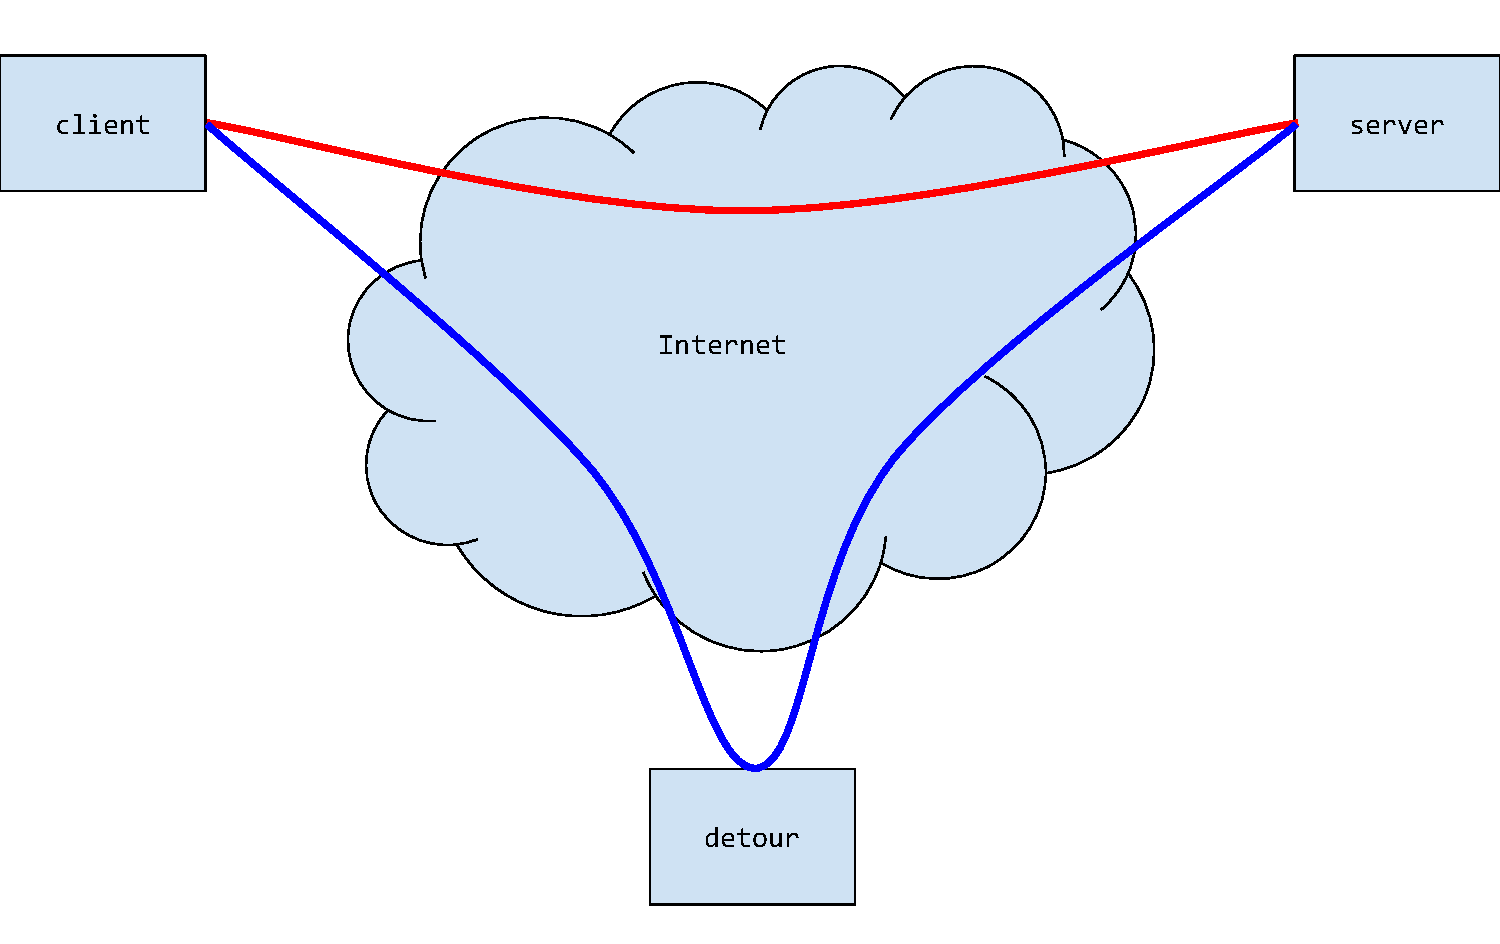
\includegraphics[width=0.8\textwidth]{figures/Concept.pdf}
  \caption{Conceptual overview of the mechanism}
  \label{fig:concept}
\end{figure}

While detour routing has been well established as a way to improve the quality
of network paths, it has proved to be something of a mirage. Finding a way to
allow everyday applications to leverage detours has been elusive. Similarly,
data striping has been an appealing avenue for performance improvements, but
applications must be designed around the concept in order to use it. As a
result, both of these concepts have remained areas of research instead of being
applied to our everyday applications.

With the advent of \ac{mptcp}, we have an opportunity to revisit detouring and
data-striping in a way that is transparent to the application. This thesis
presents a mechanism for applying detour routing to \ac{mptcp} connections. The
mechanism, illustrated in Figure~\ref{fig:concept}, establishes subflows across
detour paths. By leveraging \ac{mptcp}, our mechanism is capable of striping
data across the flows, aggregating the bandwidth of available paths. Most
importantly, since \ac{mptcp} presents the same binary-compatible OS level API
as TCP, unmodified applications may use this mechanism simply by using our
patched kernel.

We envision this system being best applied to a group of users which we refer to
as a ``Detour Collective''. These users have high-bandwidth access links, and
seek to improve application performance. By joining the collective, they offer
their computer as a detour which other members may use. In return, they gain
access to the detouring services of the other members of the collective. In
effect, the collective forms an overlay network which unmodified TCP
applications may use.

This thesis focuses only on the implementation of the mechanism for adding
detour paths to \ac{mptcp} connections. However, in Chapter~\ref{c:fw}, we will
discuss implementation issues and potential challenges for the ``Detour
Collective'', as future work for this thesis.

\section{Contributions}

The contributions of this thesis are as follows:

\begin{itemize}
\item We propose a method for leveraging detour routing in a way that is
  transparent to the application, by using \ac{mptcp}.
\item We present a prototype implementation of this method based on a system of
  Linux kernel modifications and user-space tools.
\item We evaluate this mechanism on emulated network topologies and on the
  Internet.
\end{itemize}

The remainder of this thesis has the following structure. Background information
on \ac{mptcp} and the mechanisms used in the evaluation is covered in
Chapter~\ref{c:bg}. Related work is discussed in Chapter~\ref{c:rw}. The
implementation of our system is described in Chapter~\ref{c:impl}. Experimental
evaluation is presented in Chapter~\ref{c:eval}. Finally, future work is
discussed in Chapter~\ref{c:fw} and we conclude in Chapter~\ref{c:conclusion}.

\chapter{Background}
\label{c:bg}

\section{Multipath TCP}
% Our discussion of Multipath TCP needs to be in enough depth that the reader
% understands how it works - essentially covering at least the first few pages
% of the RFC. In particular:
% - Subflows: what they are and how they work
% - How the initial subflow is created
% - How subsequent subflows are created and authenticated
% - Data sequencing and how data sequences are mapped onto subflow sequences
% - path management and data scheduling
% - ? how the linux kernel implementation is structured

Recently, multi-homed devices have become increasingly common. The most obvious
example of these devices is the smartphone, which typically comes with at least
two network interfaces: one for cellular data, and one for Wi-Fi. While these
devices have become more common, protocols have not kept up. Most Internet
traffic is carried on TCP, which identifies a data stream by the 5-tuple of
protocol, source address, source port number, destination address, and
destination port number. As a result, multi-homed devices are forced to choose
only one interface for a TCP session \cite{raiciu2012hard}. \ac{mptcp} was
designed as a protocol extension to TCP, which allows multiple interfaces (and
as a result, network paths) to be used in the same TCP stream.

\subsection{Design Considerations}
\label{sec:mptcp-design}

\ac{mptcp} has several design goals, outlined in \cite{rfc6182}. At a high
level, it aims to use the existence of multiple paths to improve efficiency and
resiliency of standard TCP. Other transport protocols support similar high-level
goals, such as SCTP with Concurrent Multipath Transfer
\cite{iyengar2006concurrent}. However, SCTP cannot easily be used as a
replacement for TCP, because applications require modification to use SCTP, and
some \acp{nat} and firewalls do not support SCTP \cite{barre2011multipath}. In
contrast, \ac{mptcp} aims to be compatible with unmodified applications and
common Internet middleboxes, so it can be deployed widely.

\ac{mptcp}'s design focuses on two types of compatibility, which motivate many
of its high-level design decisions. First, application compatibility: \ac{mptcp}
must be usable by existing TCP applications without modification. Second,
network compatibility: \ac{mptcp} must be usable across the Internet today,
including across features of the modern Internet such as \acp{nat}, firewalls,
traffic normalizers, and performance-enhancing proxies (collectively referred to
as middleboxes). In the design of \ac{mptcp}, consideration is made for the
following types of disruption by middleboxes \cite{rfc6182}:

\begin{itemize}
\item Home routers often perform \ac{nat}, and so addresses may not be the same
  on either side of a connection \cite{rfc3022}.
\item Some \ac{nat} boxes will additionally rewrite content of some protocols,
  such as URLs in HTTP \cite{rfc6182} and IP addresses and ports in FTP
  \cite{raiciu2012hard}.
\item Some middleboxes perform sequence number randomization
  \cite{hesmans2013tcp,medina2005measuring}.
\item Some middleboxes strip IP and TCP options from packets, although TCP
  options are more commonly respected \cite{medina2005measuring}.
\item Some middleboxes (especially traffic normalizers) will not allow ``holes''
  in TCP sequence numbers \cite{hesmans2013tcp}. That is, some middleboxes
  expect to see all data segments which have been acknowledged.
\item TCP segments may be broken up or coalesced \cite{hesmans2013tcp}. For
  example, TCP Segmentation Offload is a feature supported by some NICs, which
  advertises a large MSS value to the TCP stack, and then splits large segments
  into smaller ones in hardware. TCP options on these segments must be
  constructed in a way that this process will not make the data uninterpretable.
\end{itemize}

Finally, an additional network compatibility requirement is that \acl{mptcp}
``do no harm'' to existing TCP flows \cite{rfc6182}. As a result, several
congestion control mechanisms are proposed, aiming to prevent \ac{mptcp} from
using more resources than a single TCP flow would across a shared bottleneck
\cite{rfc6356,draft-olia,draft-balia,draft-wvegas}.

These combined architectural guidelines not only make \ac{mptcp} suitable for
deployment, but they also make it more resilient to the mechanisms used in this
thesis (such as \ac{nat}) to extend it in new ways.

\subsection{Architecture}

\begin{figure}[h]
  \centering
  \begin{multicols}{2}
    \begin{bytefield}{16}
      \wordbox{1}{Application} \\
      \wordbox{1}{TCP} \\
      \wordbox{1}{IP}
    \end{bytefield}
    \begin{bytefield}[bitwidth=1.1em]{16}
      \wordbox{1}{Application} \\
      \wordbox{1}{MPTCP} \\
      \bitbox{8}{Subflow (TCP)} & \bitbox{8}{Subflow (TCP)} \\
      \bitbox{8}{IP} & \bitbox{8}{IP}
    \end{bytefield}
  \end{multicols}
\caption[Comparison of TCP and \acs{mptcp} Protocol Stacks]{Comparison of
  Standard TCP and \ac{mptcp} Protocol Stacks. Originally from \cite{rfc6824}}
  \label{fig:layers}
\end{figure}

To achieve the goals described in Section~\ref{sec:mptcp-design}, \ac{mptcp} is
located between TCP and the application layer, as shown in
Figure~\ref{fig:layers}. TCP ``subflows'' are created along every path. Each
subflow looks like a normal TCP connection, but with some additional options,
and slightly different semantics.

An \ac{mptcp} connection begins with a three-way handshake, similar to a regular
TCP connection. If both hosts are capable and willing to use \ac{mptcp}, they
include a TCP option with bype \texttt{MP\_CAPABLE} on all packets of the
handshake. Additional TCP connections may be created between the two hosts once
the initial connection is established, using the \ac{mptcp} option type
\texttt{MP\_JOIN}. To authenticate this process, keys are exchanged via the
\texttt{MP\_CAPABLE} option, and a token is verified using these keys for each
new subflow via the \texttt{MP\_JOIN} option.

Either side of an \ac{mptcp} connection may establish a new subflow with its
peer at any time according to local policy. However, sometimes this may not be
possible, due to the presence of a firewall. \ac{mptcp} allows for a peer to
advertise the existence of an IP address, without creating a subflow. This is
achieved via the option \texttt{ADD\_ADDR}. Advertised addresses may be removed
with the \texttt{REMOVE\_ADDR} option. Neither option is acknowledged, so
delivery of the option is not guaranteed.

Data has sequence numbers at both the subflow level and at the connection level.
Each subflow has a \ac{dss} negotiated via the \ac{mptcp} option type
\texttt{DSS}, which maps subflow sequence numbers to data sequence numbers.
These mappings are valid for only a certain amount of bytes, and thus new
mappings must be transmitted periodically. As a result, the \ac{dss} is one
persistent form of overhead in the protocol header. Data is acknowledged both at
the subflow level (via the acknowledgment flag and field), and at the data level
(via a flag and field within the \ac{dss}).

\subsection{Implementation}

\ac{mptcp} is implemented in the Linux kernel, as well as within the XNU kernel
used by Mac OS and iOS. In this thesis, we focus on version 0.91 of the Linux
kernel implementation \cite{mptcp}. This implementation has three key features
which enable flexibility and custom policy: data schedulers, congestion control,
and path managers.

As a result of \ac{mptcp}'s flexibility in labeling data with sequence numbers,
data may be split up across multiple subflows, or even transmitted redundantly.
A data scheduler is a modular component which determines which subflow to send
application data on. The default scheduler implementation, Lowest \ac{rtt}
First, selects the subflow with the smallest \ac{rtt} and fills up its
congestion window. Other implementations include a naive round-robin scheduler
and one which sends data redundantly across each subflow. Additional schedulers
have been proposed, to mitigate problems such as head-of-line blocking and
bufferbloat \cite{paasch2014experimental}. In this thesis, we consider only the
Lowest \ac{rtt} First scheduler.

As with regular TCP congestion control \cite{rfc5681}, \ac{mptcp} congestion
control is implemented as a modular component of the Linux kernel. While normal
TCP congestion control algorithms (such as the Linux default, CUBIC
\cite{ha2008cubic}) may be used on each subflow, several \ac{mptcp} specific
implementations are provided: \ac{lia} \cite{rfc6356}, \ac{olia}
\cite{draft-olia}, \ac{wvegas} \cite{draft-wvegas}, and \ac{balia}
\cite{draft-balia}. In this thesis, we only consider \ac{lia} congestion
control, as it is the default implementation, and currently is the recommended
safe congestion control in the \ac{mptcp} specification \cite{rfc6824}.

In order to decide when to create and destroy new subflows, as well as advertise
alternative addresses, the Linux implementation uses another modular component
called a ``path manager'' \cite{mptcp}. The default implementation does nothing
(except accepting incoming connections). The Linux implementation also includes
an \texttt{ndiffports} path manager, which initiates up to $N$ subflows with a
server, from different TCP source ports. This path manager can be useful for
\ac{ecmp}, as we discuss in Section~\ref{sec:ecmp}. A \texttt{fullmesh} path
manager establishes subflows between every pair of client addresses and
advertised server addresses. A major part of the implementation of this thesis
is a path manager for the Linux kernel \ac{mptcp} implementation.

% Netfilter and Netlink?
% OpenVPN?

\section{Mininet}
\label{sec:mn}

In the evaluation of our mechanism, we use the Mininet \cite{mininet} framework
to emulate a network topology and evaluate performance across the emulated
network. Although this framework is not new in the literature of \ac{mptcp}
measurement studies \cite{paasch2013benefits,paasch2014experimental}, we use
this section to give a brief overview of its operation.

Mininet is a software-defined networking tool that allows the creation of
virtual networks. Networks created within Mininet use the native OS network
stack, and can run applications unmodified using the virtual network. However,
they do not require the full overhead of virtual machines, which emulate an
entire guest operating system and any virtual hardware used by the guest.
Instead, Mininet nodes are simply process groups using the host operating system
to access either real network devices, or virtual ones.

Mininet works by leveraging the lightweight virtualization mechanisms that the
Linux kernel provides. Within the kernel, \emph{namespaces} are used to organize
and partition the resources a process (or group of processes) can see and use.
For instance, mount namespaces limit an application's view of the file system.
PID namespaces give a group of applications a new set of process identifiers,
starting from 1. Similarly, network namespaces group the resources of the
operating system network stack. In particular, network namespaces group network
interfaces, as well as routing tables and firewall rules. Kernel namespaces are
the foundation of modern lightweight virtualization tools such as Docker
\cite{merkel2014docker}.

Network namespaces may be connected by virtual Ethernet pairs, such that traffic
sent on a virtual interface on within one namespace can be received on a virtual
interface within another. Furthermore, these virtual Ethernet links may be
configured using the Linux Traffic Control framework, to emulate packet loss,
latency, jitter, reordering, packet duplication, and control link bandwidth.

Mininet creates virtual networks via the following mechanism
\cite{lantz2010network}. Each host is a shell process running within a separate
network namespace. Hosts share a pipe to the Mininet parent process, over which
commands and output are exchanged. Links are virtual Ethernet pairs. Switches
may be emulated using userspace or kernel OpenFlow switch implementations,
although we did not use switches in our experiments.

As a network emulation framework, Mininet presents several attractive qualities.
It is more lightweight than virtual machines, enabling practical experimentation
on single machines. It provides an easy-to-use Python API, reducing manual
interaction in the experimentation process. By providing complete virtual
machine images with Mininet and experiments pre-installed, experiments may be
made completely reproducible, and distributed easily online \footnote{Virtual
  machine images and data for our experiments will be made available at:
  \url{https://brennan.io/thesis}}. Finally, as compared to larger, hardware
based emulation frameworks such as EmuLab\cite{hibler2008large}, the development
time and debugging time can be dramatically reduced when constructing
experiments.

\chapter{Related Work}
\label{c:rw}

The mechanism in this thesis involves adding alternative routes to a connection,
in order to improve connection performance. This can be seen as related to
several concepts in the body of networking research: multipath routing, overlay
routing, source routing, channel bonding, and proxying. In this chapter, we will
examine related work at each relevant level of Internet.

\section{Link Layer}
\label{s:rw-ll}

At the link layer, aggregating multiple low-capacity links to create a single,
virtual link with higher capacity is called \emph{inverse multiplexing}, or
sometimes channel bonding \cite{duncanson1994inverse}. Linux provides a bonding
driver which allows this to be done in software, presenting a single virtual
interface to the host machine. Unfortunately, this mechanism typically requires
identical links and configuration on either side of them, limiting the use of
these setups \cite{chiussi1998generalized}.

Another interesting approach to bandwidth aggregation, falling somewhere between
the link layer and the network layer, is the ``Beyond One's Bandwidth (BOB)''
system \cite{radio-agg}. This system, designed for use on residential wireless
access points, allows neighboring residential access points to share bandwidth.
Each router negotiates a connection with its neighboring access points, and uses
round-robin scheduling to assign packet flows to different gateways. Streams,
like TCP, must remain on the gateway that their initial packet used, so the
system does not truly aggregate bandwidth for streams, but instead
load-balances. The authors considered implementing a \ac{mptcp} proxy with
subflows over each gateway, but rejected this strategy since it required an
egress point on the wide area Internet \cite{radio-agg}.

In the case of link layer approaches to bandwidth aggregation, most mechanisms
are highly localized. Channel bonding approaches are limited to multiple links
between the same endpoints, and these links require identical hardware
\cite{chiussi1998generalized}. Beyond One's Bandwidth is only applicable to
wireless access points within range of each other. Our mechanism allows
bandwidth aggregation across entire paths, not simply nearby links.

\section{Network Layer}

Improved Internet routing has been a goal for researchers for a long time, and
the network layer has been a natural place to begin. Related work includes
source routing, overlay routing schemes, and several improved routing
approaches, many of which involve multipath routing.

\subsection{Source Routing}

A major part of this thesis (and many other studies) involves specifying
``waypoints'' or detour hosts that a packet must traverse before it continues on
to its final destination. Although packets are normally routed on the Internet
hop-by-hop, there are mechanisms for specifying the path that a packet should
take. In IPv4, these mechanisms are the options \ac{lsrr} and \ac{ssrr}
\cite{rfc791}. These IP options allow the source of a packet to specify a
partial (Loose) or complete (Strict) route consisting of a list of addresses.
The route taken is recorded within the packet, and reply packets must follow the
same route. In IPv6, a similar mechanism called Segment Routing is being
proposed by the IPv6 Maintenance Working Group of the IETF
\cite{draft-segment-routing}.

Source routing options are considered insecure. If source routing options were
respected, an attacker could send a packet with a complete route specified,
while spoofing the source address. Reply packets would follow the recorded route
in reverse back to the attacker \cite{bellovin1989security}. This behavior would
allow complete spoofing of source addresses, including receiving reply packets.
Furthermore, maliciously crafted source routes can be used to create bandwidth
exhaustion attacks and evade firewalls \cite{rfc7126}. As a result, it is
recommended that routers and firewalls drop packets bearing these options, and
many routers on the Internet do \cite{rfc7126}.

Detour routing is simply one-hop source routing. If source routing options were
widely supported on the Internet, our mechanism might be able to use them to
route subflows across detours. Such an implementation would require no
modification of a detour host. However, the security implications of source
routing on the Internet heavily outweigh their potential benefits. As a result,
we must resort to other mechanisms to perform the same function as source
routing, such as tunneling and \ac{nat}.

\subsection{Overlay Routing}

An alternative to designing and deploying a full new network layer protocol is
experimenting on overlay networks. Overlay networks are networks constructed on
top of an existing ``substrate'' network. Nodes route traffic among each other
using the substrate network rather than direct links. Traffic is routed through
a sequence of overlay nodes before reaching the final destination, rather than
being directly routed through the substrate. In the case of the Internet, these
networks can be advantageous because they can add functionality that is not
widely deployed (such as multicasting) and they can make routing decisions based
on more information than the Internet.

Several overlay network approaches have been proposed and deployed. An early
example, the M-Bone, connected networks capable of multicasting via tunnels
\cite{mbone}. This allowed multicasting even though the Internet as a whole did
not support it. Later approaches, such as Overcast \cite{jannotti2000overcast},
apply the concept of overlay networking at the application level to achieve
similar results.

Andersen \textit{et al.}~\cite{ron} describe \ac{ron}, a framework for creating
overlay networks and routing traffic along them. Applications link to a
user-space library, and access the network via a \texttt{send} function and a
\texttt{recv} callback. Applications may choose to send via the default Internet
routed path, or via the overlay. Routing is performed at each node, rather than
at the source. The routing algorithm takes into account several virtual link
characteristics, as well as application-specified metrics, which are stored in a
database.

The design goal of \ac{ron} is to improve reliability by using overlays. The
result also showed that latency and throughput could be improved via overlays.
However, as an application-level approach, \ac{ron} cannot be applied to
unmodified applications. Andersen \textit{et al.} later described a redundant
routing scheme in which redundant copies of packets are sent along multiple
paths \cite{andersen2003best}. They compared this approach with a more
traditional approach that reacts to link failures and routes around them,
similar to the \ac{ron} framework's original routing system. However, they did
not attempt to use multiple paths without redundancy, since their study focused
on loss rates rather than throughput.

Another extension of the \ac{ron} framework attempted to use a biologically
inspired approach to multi-path routing \cite{leibnitz2006biologically}. Their
mechanism discovers routes via an iterative broadcasting method, not unlike the
construction of a shortest path tree. When a selection of routes is ready, the
mechanism moves into a route maintenance mode. A main route is selected, with
alternative routes being used as backups. Packets are transmitted along the main
route with a high probability, and along the backup routes with low probability.
Based on changes in link state, as well as some degree of randomness, the main
route may become backup, while a different route is selected as the main route.
The authors do not measure bandwidth aggregation, as their main focus is
resilience against link failures.

Gummadi \textit{et al.} \cite{gummadi2004improving} demonstrated a simpler
approach to detour routing. Rather than creating a full overlay network in which
each node monitors links and maintains routing tables, they applied source
routing. They designed \ac{sosr}, a system which tunnels traffic to an
intermediary, which then forwards the traffic on to the destination. The
intermediary performs \ac{nat}, so that reply traffic is forwarded back to the
destination. Using \ac{sosr} and randomly selected PlanetLab intermediaries,
they were able to recover from 56\% of failures on the paths to popular web
servers. However, they did not report the throughput of \ac{sosr} paths. In this
thesis, we use an approach similar to Gummadi \textit{et al.} in simply
tunneling traffic across a chosen intermediary, rather than constructing a
complete overlay network.

As far as we could find, there are no overlay routing systems which attempt to
correct Internet routing inefficiencies by combining multiple paths without
redundancy. However, transport-layer systems based on overlay networks have been
created which do so (see Section~\ref{s:rw-transport}).

\subsection{Equal Cost Multi-path Routing}
\label{sec:ecmp}

The \ac{mptcp} protocol specification allows for subflows to be established
between the same two IP addresses as a pre-existing subflow in a connection,
using a different TCP source port \cite{rfc6824}. One reason this is allowed is
to enable path diversity via \acf{ecmp}. In large data center networks, highly
redundant network topologies have been deployed, so that there are several
routes between hosts. Routers in these topologies use \ac{ecmp} to choose
between paths that have the same cost, by hashing the connection 5-tuple
\cite{raiciu2011improving}. While normally, \ac{ecmp} provides load-balancing,
it can be combined with \ac{mptcp} to provide bandwidth aggregation, since a
subflow's different 5-tuple may result in a different route. Raiciu \textit{et
  al.} \cite{raiciu2011improving} describe in detail a simulation study that
evaluates the performance of \ac{mptcp} on several data center topologies and
congestion controls. They also describe a validation on an Amazon EC2 data
center with a highly redundant topology, in which using \ac{mptcp} with four
subflows achieved a 3x throughput improvement.

Similar to source routing, \ac{ecmp} offers the capability for the source of a
packet to alter the route its packet takes. Unlike source routing, \ac{ecmp}
gives only very loose control: by altering the source port (and thus the
connection 5-tuple), a second TCP flow (or subflow) \textit{may} take a new
route, but it may not. Using several subflows improves the probability of
alternative routes being used. If \ac{ecmp} were common outside of datacenter
networks, it would be possible to use separate source ports and obtain different
routes for subflows, replacing our detour mechanisms. However, this is not
currently possible on the Internet.

\subsection{Binder}

Another application of \ac{mptcp} to bandwidth aggregation is Binder, a system
for aggregating the bandwidth of several Internet gateways \cite{binder}. This
mechanism was developed in an area of rural Scotland, containing several
low-bandwidth gateways. Rather than use one gateway primarily and others as
backup, Binder allows aggregation of all of the gateways.

This is achieved by routing all outgoing traffic through an OpenVPN connection.
Binder leverages the capability of OpenVPN to run over \ac{mptcp}. One subflow
is dedicated to each gateway (using IP source routing options). The OpenVPN
server, located outside of the local network, terminates the \ac{mptcp}
connection and performs \ac{nat}, routing all packets to their final
destinations.

We consider this to be a network layer mechanism since it forwards IP datagrams
over the OpenVPN connection. As pointed out in their paper, Binder strikingly
parallels channel-bonding techniques such as the ones described in
Section~\ref{s:rw-ll}.

Our mechanism also uses OpenVPN, as one of the two implementation alternatives
for the detour. However, a key difference is that while Binder uses OpenVPN over
\ac{mptcp}, we only put a single subflow of an \ac{mptcp} connection through
OpenVPN, essentially leveraging OpenVPN for tunneling. Furthermore, while Binder
enables bandwidth aggregation, it does not leverage source routing, as our
system does. Finally, Binder is a system which operates at a network gateway,
while ours operates on a client host itself.

\section{Transport Layer}

\subsection{mTCP}
\label{s:rw-transport}

\ac{mptcp}, the heart of our mechanism, is at the transport layer. It is built
on several years of research and development, and the literature is full of work
related to the development of multipath transport algorithms. Overviews of these
prior works can be found in \cite{barre2011multipath,raiciu2012hard}. Most of
these works are based on multi-homed devices, and thus not directly related to
this thesis.

However, one prior transport-layer approach is very relevant. In
\cite{zhang2004transport}, Zhang \textit{et al.} describe the implementation of
mTCP, an early multipath variation of TCP. Rather than using a TCP connection
per-subflow, mTCP simply routes TCP segments across different paths. Congestion
control is performed separately on each ``subflow'', while the receive window is
global. Acknowledgements are transmitted on only one return path. Paths are
dynamically added based on a heuristic that involves an estimated path
disjointness metric based on the measured route and path latency. Paths are
suppressed when shared congestion is detected, and removed if they are detected
to have failed.

The mTCP mechanism is based on a user-space TCP implementation, and it uses
\ac{ron} \cite{ron} as a network layer capable of providing multiple routes. By
using \ac{ron}, single-homed devices are just as capable of using mTCP for
bandwidth aggregation as multi-homed devices. However, due to the nature of mTCP
as a fully user-space library, the mechanism cannot be made compatible with
unmodified applications. Additionally, its design choices contradict many of the
network compatibility considerations made in the design of \ac{mptcp}. In the
years since mTCP was designed, \ac{mptcp} has been standardized, with the
benefits of improved network and application compatibility. We view this thesis
as a more compatible and standards-based take on the concepts of mTCP. Our
mechanism has the benefit of transparency to the application, and no dependence
on \ac{ron}.

\subsection{MPTCP Proxying}

A recent \ac{mptcp} IETF working group draft proposes a set of proxying
mechanisms that allow ISPs to improve client TCP and \ac{mptcp} connection
throughput \cite{boucadair-mptcp-plain-mode-10}. Based on observations that
\ac{mptcp} server deployment has not been strong, these mechanisms expect a
server and optionally a client which do not support \ac{mptcp}. They proxy
traffic through \acp{mcp}, devices which ISPs deploy throughout the network.
There are two possible deployment scenarios: one \ac{mcp} and two \ac{mcp}.

In the one \ac{mcp} scenario, an \ac{mptcp}-enabled client would like to use
\ac{mptcp} to connect to a server which does not support it. It establishes a
connection to a \ac{mcp}, specifying the final destination within the
\texttt{SYN} segment. It may then establish additional subflows to the \ac{mcp}
using its other interfaces. The \ac{mcp} proxies the connection data to the
final destination via a plain TCP connection.

In the two \ac{mcp} scenario, both the client and server are not \ac{mptcp}
enabled. Instead, a TCP connection bearing an \texttt{MP\_CONVERT} TCP option is
routed through the ISP, to an \ac{mcp}. The \ac{mcp} establishes a \ac{mptcp}
connection to another \ac{mcp}, which will then connect to the final destination
over TCP.

There is some overlap in the goals of this IETF proxy mechanism, when compared
to our detouring mechanism. Both aim to bring the benefits of \ac{mptcp} to
devices which otherwise may not be able to use them. The proxy mechanism focuses
on servers, and possibly clients, which do not support \ac{mptcp}. Our detouring
mechanism instead focuses on single-homed devices which support \ac{mptcp}, but
have no additional addresses to create new paths along. These approaches are not
mutually exclusive. In fact, the one \ac{mcp} scenario could be used in
conjunction with our mechanism to allow single-homed devices to gain the
benefits of multiple paths, even when a server does not support \ac{mptcp}.

\section{Application Layer}

The application layer is well suited to allow experimentation, and is an
excellent breeding ground for building new concepts. Applications may be
modified and updated at a much quicker pace than the development of network and
transport layer protocols can occur. As a result, the application layer
demonstrates a diverse set of mechanisms for using multiple paths and
aggregating bandwidth. We describe some of these mechanisms in this section.

\subsection{Peer to Peer File Sharing}

Peer to peer file sharing systems are typically distributed in their nature.
Centralized systems require communication with a single server, and thus
communication along only one path. An the other hand, peer to peer systems
frequently involve communicating with several peers simultaneously, each one
along a different path. As a result, peer to peer systems can enable bandwidth
aggregation very naturally.

An early peer to peer system, Gnutella \cite{adar2000free}, resembles an
application-layer overlay network. Peers join the network by connecting to
several well-known peers, and receiving information about other peers. They may
then broadcast queries to peers, which are forwarded throughout the overlay
network. Replies are forwarded along the reverse path, and contain information
for peers to establish a direct connection, in order to exchange files. The
actual file exchange is made directly between peers over \ac{http}, and thus is
only a single-path exchange.

Later systems, such as BitTorrent \cite{cohen2003incentives}, allow data to be
exchanged via the overlay network itself, leveraging bandwidth aggregation. In
BitTorrent, files are broken into small chunks which may be requested from any
peer which has the chunk. Peers are incentivized to upload portions of the file
which they possess because other peers will ``choke'' them (stop uploading to
them) if the exchanges are not mutually beneficial. By communicating with
multiple peers at a time, BitTorrent is capable of aggregating the bandwidth of
several Internet paths.

Both of these technologies, and many other peer to peer systems, enable powerful
content distribution mechanisms, but are not ultimately applicable to other
unmodified applications. Live streaming versions of BitTorrent exist, both in
research \cite{mol2009design} and in commercial applications
\cite{ruckert2014clubbing}. However, BitTorrent is not applicable to
communications which do not involve swarms of users, such as video calling. In
general, while peer to peer solutions can be very powerful, their application
layer design limits the scope of their utility.

\subsection{HTTP Range Requests}

\ac{http} is a ubiquitous application layer protocol for accessing web pages.
HTTP 1.1 \cite{rfc2616}, contains an optional feature known as range requests
\cite{rfc7233} which allow a client to request a byte range of a file. This
allows clients to resume interrupted transfers or to retrieve partial contents,
such as a page from a larger document.

Kaspar \textit{et al.} \cite{kaspar2010enhancing} describe the use of \ac{http}
range requests to download large files over multiple wireless interfaces. Their
mechanism requests separate ranges on each wireless interface and reassembles
them locally. Their mechanism focuses on live media playback, and so it seeks to
minimize start-up time while aggregating throughput. However, their mechanism is
applicable to regular \ac{http} downloads as well.

Similar to peer to peer networks, this approach cannot be generalized to other
applications. However, \ac{http} is a very common protocol, and a bandwidth
aggregation approach for \ac{http} could be very widely applicable.
Unfortunately, Kaspar \textit{et al.}'s approach only makes use of multiple
network interfaces as sources of alternative routes, similar to plain
\ac{mptcp}. Their mechanism could be extended to use detour routes, provided
that detours run \ac{http} proxies which support range requests. However, our
mechanism is also capable of using detour routing to provide alternative routes.
Being based on TCP, it is directly applicable to \ac{http}. By operating at the
transport layer, our mechanism is capable of much more fine-grained data
striping. Further, our mechanism could be applied to pipelined sessions
containing small files, while Kaspar \textit{et al.}'s approach is limited to
large files.

\chapter{Implementation}
\label{c:impl}
% Section intro:
% 1. Expectations (what hosts are there, and which ones run our code?)
% 2. Overview of the distinct pieces of software (client kernel, client daemon,
%    detour daemon)
% Subsection - Detour daemon
% Subsection - Client kernel
% Subsection - Client daemon

% smoother transition once we have everything

In this project, we implement a system which allows one host to dynamically add
new overlay routes to a Multipath TCP connection. Each overlay route is a new
subflow, which is tunneled across a third-party host. The system involves at
least three hosts:
\begin{itemize}
\item The \emph{client} is the active opener of the \ac{mptcp} connection. In
  our system, the client actively requests all detours and initiates all
  subflows.
\item The \emph{server} is the passive opener of the \ac{mptcp} connection.
\item The \emph{detour} is a host which acts as a waypoint along the overlay
  route from the client to the server. There may be more than one detour at a
  time, and there are multiple ways to implement the detour service.
\end{itemize}

We assume that the server supports Multipath TCP, and require no additional
customization for our system to work. In our current implementation, the detour
host must run some version of Linux, and the client must run a version of the
Linux kernel that is built with support for \ac{mptcp} and our path manager
patch. Additionally, the detour must run one of two user-space daemons, and the
client must also run a user-space daemon.

The system is implemented via a number of interacting components. First, a path
manager extension for version 0.91 of the Linux \ac{mptcp} implementation
\cite{mptcp}, which allows the client's kernel to request new detour paths,
receive them, and create subflows across them. Second, a user-space utility
which receives messages from the kernel and creates the necessary detour paths.
Finally, we implement two different types of detour daemons, which run on the
detour host. These components are illustrated in Figure~\ref{f:MovingParts}.

\begin{figure}[h]
  \centering
  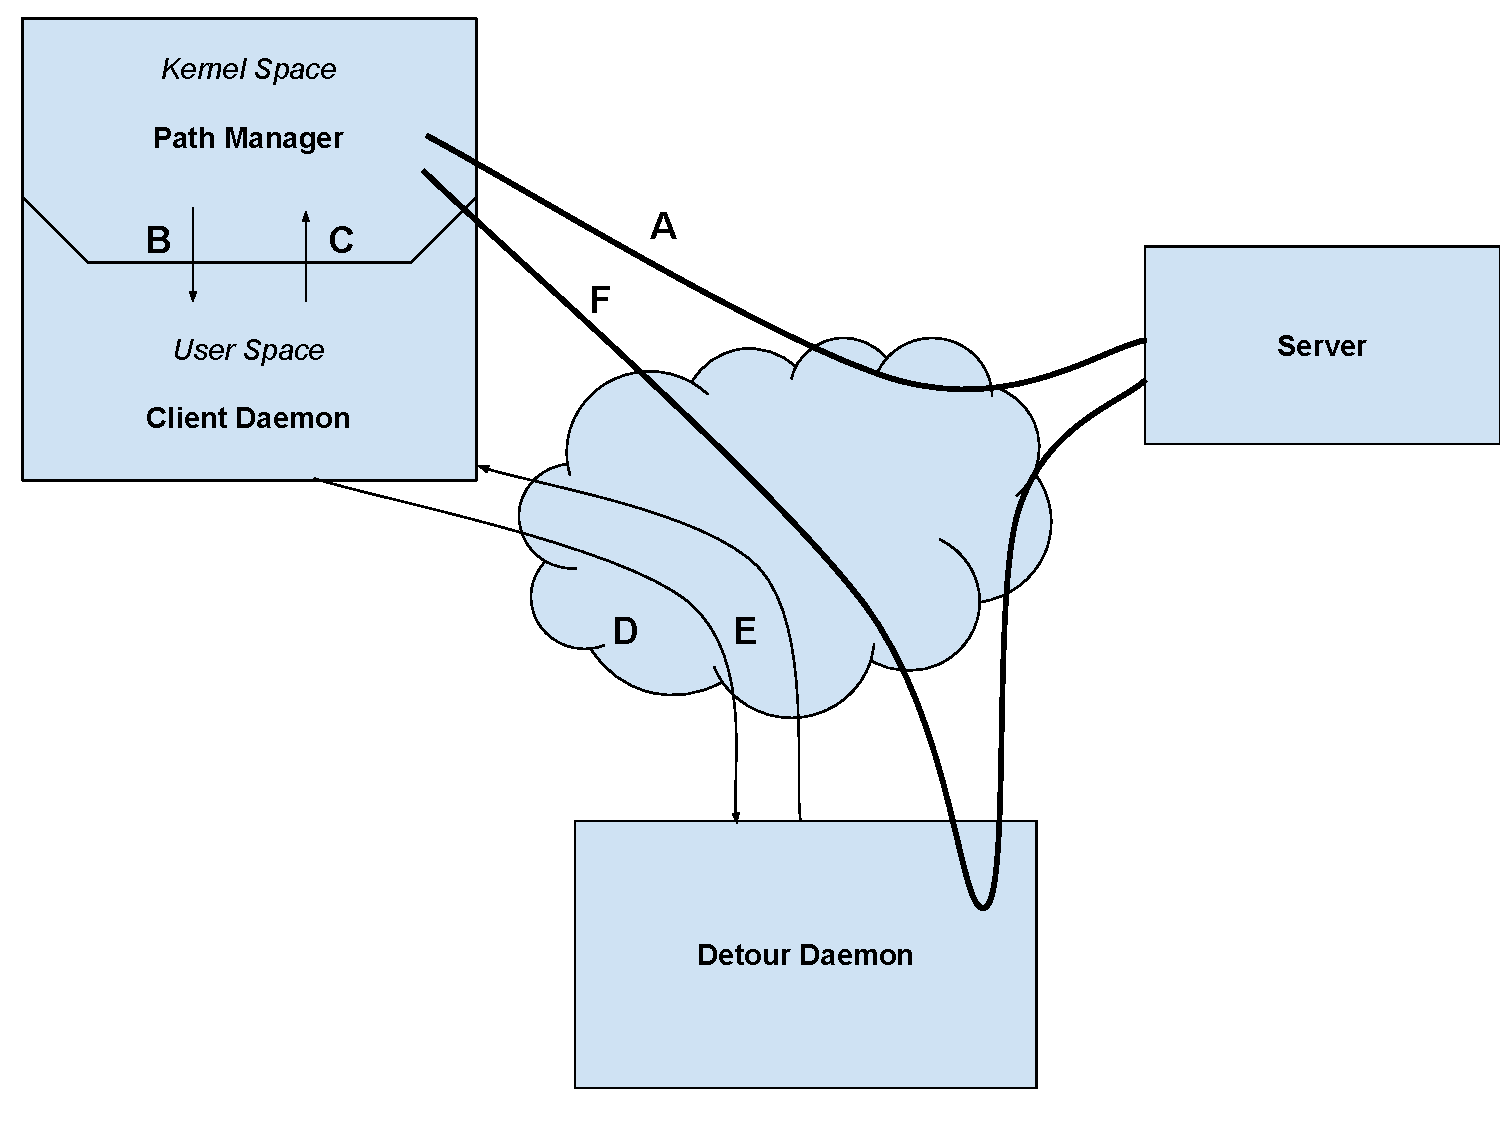
\includegraphics[width=0.8\textwidth]{figures/MovingParts.pdf}
  \caption[Interaction of client, detour, and server]{
    The components and their communications. In \textbf{A}, the initial subflow
    across the default route is created. In \textbf{B}, the path manager
    requests an overlay route. In \textbf{C}, the client daemon reports overlay
    routes back to the path managers. In \textbf{D} and \textbf{E}, the client
    and detour daemons negotiate an overlay route. In \textbf{F}, a subflow is
    created through the detour.
  }
  \label{f:MovingParts}
\end{figure}

The typical interaction of these components is as follows. First, a process on
the client creates a \ac{mptcp} connection to the server. The first subflow uses
the Internet routed path. Once this connection is fully established, the path
manager requests overlay routes on which it may create subflows. The client
detour daemon receives this request, and attempts to set up detours. The detours
are currently selected from a static configuration file. The client and detour
daemons negotiate a tunnel, which may be implemented in two different ways. The
client reports this back to the kernel, which creates subflows for the
\ac{mptcp} connection across every available detour, until a predefined limit is
reached. In our implementation, this limit is two, but it may be set by an
administrator using the \texttt{sysctl} tool.

In the remainder of this chapter, we will discuss each of these components at
length.

\section{Detour Daemon}

We have implemented two different mechanisms for tunneling \ac{mptcp} subflows across
a detour. In both cases, the detour host must run a daemon that assists in
tunneling traffic from the client to the server.

\subsection{OpenVPN Tunneling}

The first mechanism involves the open-source tool OpenVPN
\cite{yonan2007openvpn}. OpenVPN is a program which provides virtual networking
between two computers. It comes with two operating modes. The first provides a
simple virtual link between two hosts, with no other capabilities. The second
uses this virtual link to create a virtual network. One host is the server,
which provides IP addresses and routes traffic among clients and the rest of the
Internet. OpenVPN also provides encryption and PKI-based authentication
services. Our detour runs OpenVPN as a server in the second mode of operation,
configured as follows:

\begin{itemize}
\item The connection is over UDP, to avoid the so-called ``TCP Meltdown'' effect
  caused by two sets of TCP timers and congestion control algorithms interfering
  with each other when TCP is tunneled through TCP \cite{khanvilkar2004virtual}.
\item The initial connection negotiation requires the client and server to
  exchange certificates. This mutual authentication process could be used to
  protect both the client and detour from working with a peer that is not a
  member of their ``Detour Collective''. Further, the certificate can be used to
  provide accountability for the origin of detoured traffic, lowering the risk
  to a detour server. These applications of certificate verification are
  discussed further in Chapter~\ref{c:fw}.
\item Subsequent messages are not protected by encryption or signatures, to
  reduce per-packet space and time overhead. In the case of a malicious detour,
  these cannot provide any additional security, because traffic would be
  decrypted at the detour before forwarding.
\end{itemize}

Clients connect to this VPN, creating a virtual network interface. The client
receives a routing rule from the detour advertising that it can reach all hosts
on the Internet with a high cost. As a result, the client operating system will
prefer other routes instead of the VPN. However, the route is available for the
path manager to route subflows along.

One important aspect of VPN configuration is that the detour must create a
private IP subnet. It provides a DHCP service \cite{rfc2131} to assign IP
addresses to clients as they connect to the VPN. Clients are expected to be able
to connect to multiple detours simultaneously. To do this without conflict, each
detour must use a distinct private IP subnet, so that there is no chance of the
client addresses overlapping, and also so that the gateway address of the VPN is
unique on the client.

In a large-scale implementation of this technology, these subnet allocations
could be handled by a centralized detour management server, or an appropriate
distributed protocol among the detours. The 10.0.0.0/8 subnet is reserved for
private networks, and if each detour were to establish its own /24 subnet, there
would be capacity for 65,536 non-conflicting subnets. A random subnet and IP
allocation may also be sufficient. Collisions in IP namespaces would render a
detour unusable for a particular client. However, in a situation with enough
detours to make collisions likely, many alternative detours would exist for a
client to fall back on. In our testing, subnets were manually allocated to avoid
conflicts.

Finally, in order to forward VPN traffic to the Internet, the detour must be
configured (via Netfilter) to perform network address translation (\ac{nat}) on
outgoing packets. This process is typical for a home router and for VPNs which
provide Internet access \cite{rfc3022,yonan2007openvpn}. As discussed earlier,
\ac{mptcp} is designed with this behavior in mind, and so it is capable of
functioning through \ac{nat}, so long as the middleboxes do not remove TCP
options in transit, or modify data contents \cite{rfc6182}.

The OpenVPN implementation has several attractive qualities. First, it relies on
a well-used protocol for forwarding traffic. Second, an established OpenVPN
connection may be used as a detour for any server address and port number,
without any additional setup. The NAT mechanism discussed in
Section~\ref{sec:nat} requires communication with the detour server for every
new server address and port number combination. A final benefit of the OpenVPN
mechanism is that it provides a built-in mechanism for mutually authenticating
the client and detour. However, there are some drawbacks. Since packets are
tunneled, at least 28 bytes of overhead (IP and UDP headers) are required. To
avoid fragmentation, the connection's maximum segment size (MSS) may need to be
manually adjusted. In our testing, the maximum segment size was automatically
adjusted by OpenVPN without need for manual modification.

\subsection{NAT Tunneling}
\label{sec:nat}

The second approach directly modifies packet source and destination addresses,
without actually using a protocol (like OpenVPN) for tunneling. Rather than
encapsulate packets and send them to the detour, the client daemon instead
informs the detour of the intended destination, and requests that it perform
\ac{nat} on its packets. Then, the kernel addresses packets directly to the
detour, on an agreed upon port. The detour forwards these to the final
destination, and forwards reply packets to the client. On packets destined to
the server, the detour rewrites the destination address and port number to be
the server's, and rewrites the source address and port number to be its own. For
reply packets, the detour rewrites the destination address and port number to be
the client's, and rewrites the source address and port number to be its own. In
order to arrange these \ac{nat} mappings, clients use a simple signaling
protocol based on UDP.

\begin{figure}
  \centering
  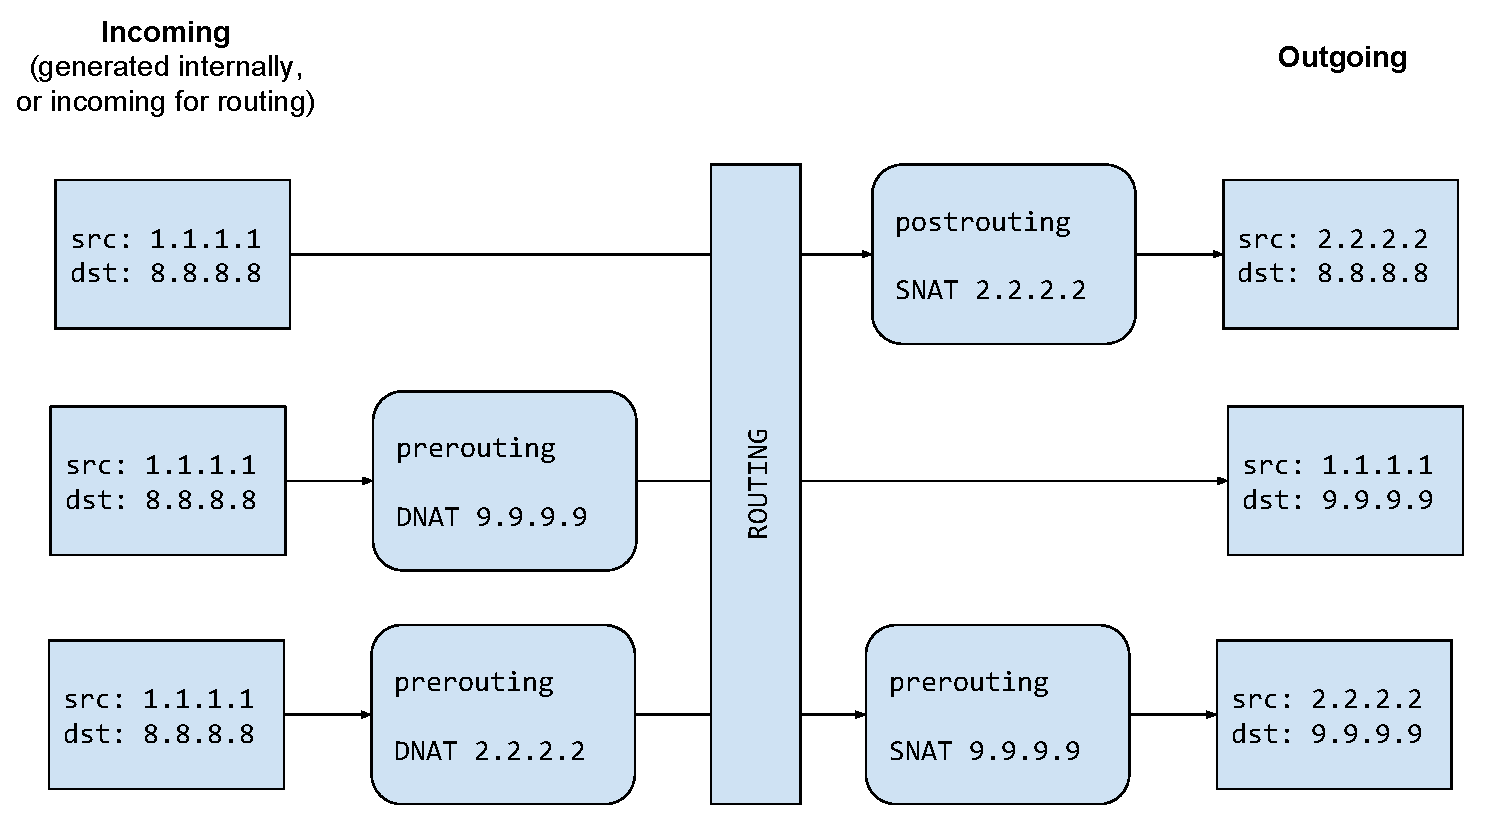
\includegraphics[height=0.3\textheight]{figures/NATTypes.pdf}
  \caption[Types of \ac{nat} provided by Netfilter]{Types of \ac{nat} provided
    by Netfilter. \textbf{Top:} SNAT only. \textbf{Middle:} DNAT only.
    \textbf{Bottom:} Both SNAT and DNAT, as used in the NAT tunnel.}
  \label{fig:NATTypes}
\end{figure}

The Linux kernel's Netfilter framework allows for two types of \ac{nat},
illustrated in Figure~\ref{fig:NATTypes} \cite{russell2002nat}. The first kind,
source \ac{nat} (SNAT), rewrites the source address of the packet. This is the
typical form of \ac{nat} used by home routers: the source address of each
outgoing packet is rewritten to be the router's external IP address, but the
destination is unchanged \cite{rfc3022}. This type of rule is applied after
routing has taken place. The second kind of \ac{nat} supported by Netfilter is
destination \ac{nat} (or DNAT) which rewrites the destination of the packet.
This rule is applied before routing, so that a proper interface can be selected
for the new address.

The detour takes advantage of both forms of \ac{nat} offered by the kernel.
First, it applies DNAT, setting the destination address to be the final server's
IP address (signaled ahead of time). Then, it applies SNAT, setting the source
address to be its own external IP. The Netfilter framework remembers these
connections so that reply packets are properly forwarded back to the client.
Thanks to Netfilter, this \ac{nat} mapping can be arranged with two
\texttt{iptables} commands, with no custom kernel or user-space code required
for packet forwarding.

As mentioned earlier, the server address must be communicated to the detour
ahead of time in order to use this scheme. To that end, we have designed a
simple UDP-based protocol for clients to request \ac{nat} mappings from a
detour. The detour listens for requests on UDP port 45672. The request format is
shown in Figure~\ref{fig:udp-nat-packet}.

\begin{figure}
  \centering
  \begin{bytefield}[bitwidth=0.6em]{32}
    \bitheader{0,7,8,15,16,23,24,31}\\
    \bitbox{8}{\texttt{ver}} & \bitbox{8}{\texttt{op}} & \bitbox{16}{\texttt{reserved}} \\
    \wordbox{1}{\texttt{rip}} \\
    \bitbox{16}{\texttt{rpt}} & \bitbox{16}{\texttt{dpt}} \\
  \end{bytefield}
  \caption{UDP \ac{nat} tunnel request structure}
  \label{fig:udp-nat-packet}
\end{figure}

The \texttt{ver} field is a protocol version, currently set to 1. The
\texttt{op} field contains the operation of this message: request (0) or
response (1). The \texttt{reserved} field is unused, providing padding for the
request. In the future, this field could be used for flags that enable IPv6
support. Since there are several IP addresses and ports involved in the
tunneling setup, we will define them each before defining the remaining fields
of the message.

\begin{itemize}
\item Client IP address, port number: the IP address of the client, and the
  client-side port number, which is usually ephemeral.
\item Detour IP address, port number (client side): the IP address and port
  number that the client will address its communication to.
\item Detour IP address, port number (remote side): the IP address and port
  number which are used when the detour opens its corresponding connection on
  the remote.
\item Remote IP address, port number: the IP address and port number of the
  server.
\end{itemize}

The fields \texttt{rip} (short for ``remote IP address'') and \texttt{rpt}
correspond to remote IP address and port number. The \texttt{dpt} field
corresponds to the detour port number, client side. In a request, the client
proposes a \texttt{dpt} (usually the same as the \texttt{rpt}). In the response,
the detour specifies the port number which will actually be used. Semantically,
the detour creates a mapping from the pair (client IP address, \texttt{dpt}) to
the pair (\texttt{rip}, \texttt{rpt}). The detour may alter the proposed
\texttt{dpt} field for several reasons:

\begin{itemize}
\item A tunnel to the (\texttt{rip}, \texttt{rpt}) pair is already open for that
  client IP address, using a different \texttt{dpt}. Rather than create a new
  (client IP address, \texttt{dpt}) pair which maps to the same (\texttt{rip},
  \texttt{rpt}) pair, the detour may wish to return the \texttt{dpt} of the
  existing mapping.
\item The (client IP address, \texttt{dpt}) pair already maps to a different
  (\texttt{rip}, \texttt{rpt}) pair. A new \texttt{dpt} is returned to avoid a
  conflict.
\item The detour may have a socket listening for connections on the proposed
  \texttt{dpt} (such as an HTTP server on port 80), and so it may wish to avoid
  creating a tunnel which would prevent the client from accessing that service.
\end{itemize}

The client port number is not used in the mapping, to allow the client to create
several subflows to the same server through the detour (potentially on separate
\ac{mptcp} connections). This also avoids race conditions in which a client port
number is proposed, but then used by the operating system while waiting for the
detour's response.

In order to create the tunnels, the detour runs two IPTables commands, which
create \ac{nat} rules. The first performs DNAT:

\begin{minipage}{\linewidth} % avoid line breaks
\begin{lstlisting}
iptables -t nat -A PREROUTING \
         -s (*\emph{ClientAddress}*) \
         -d (*\emph{DetourAddress}*) \
         -p tcp --dport (*\emph{DetourPort}*) \
         -j DNAT --to (*\emph{RemoteAddress}*):(*\emph{RemotePort}*)
\end{lstlisting}
\end{minipage}

In this command, we add a rule to the \texttt{nat} table, on the
\texttt{PREROUTING} chain. Incoming packets from the client, addressed to the
detour on the agreed upon \textit{DetourPort} are sent to the \texttt{DNAT}
chain, which rewrites the destination address to be the agreed upon remote
address and port. This must occur before the kernel routes the packet. Once the
kernel has routed the packet, the SNAT rule can be applied:

\begin{minipage}{\linewidth} % avoid line breaks
\begin{lstlisting}
iptables -t nat -A POSTROUTING \
         -s (*\emph{ClientAddress}*) \
         -d (*\emph{RemoteAddress}*) \
         -p tcp --dport (*\emph{RemotePort}*) \
         -j SNAT --to (*\emph{DetourAddress}*)
\end{lstlisting}
\end{minipage}

Since the destination address and port have already been modified, this rule
looks for packets addressed to the remote address and port, but still using the
client address as the source. It jumps these packets to the SNAT chain, where
their source address will be rewritten as the detour's address.

It is important to understand that these rules are generally only applied to the
initial SYN segment of the TCP flows. Once these rules are applied, the
connection tracking mechanism of the kernel takes over, ensuring that these
rules are applied in reverse to response packets.

The detour daemon is implemented as a Python script. It listens for tunnel
requests, executes the correct commands to create them, and then sends
responses. It ensures that detour ports do not conflict with each other, or with
ports that are open on the daemon machine. It also ensures that on termination
of the detour daemon, all tunnels are torn down.

This mechanism has the advantage that it requires zero space overhead within the
packet. Since no headers are added, the full amount of data may be transmitted
in these segments. However, the disadvantage is that tunnels must be configured
each time a new \ac{mptcp} connection is created on the client. In the case of
OpenVPN, a new subflow may be tunneled through an existing OpenVPN connection
without any additional signaling with the detour. However, with the \ac{nat}
approach, each time a subflow is initiated with a new server, a tunnel must
first be negotiated with the detour server, incurring an \ac{rtt} delay.

The protocol described here is rather na\"ive. Similar to DNS, this protocol is
vulnerable to spoofing attacks for replies. Additionally, malicious clients may
use this protocol to create large amounts of detours, exhausting resources on
the detour machine. The protocol here is not intended to be secure against these
types of attacks. Rather, the protocol is designed to assess the efficacy of a
\ac{nat} based approach. It is the subject of future work to design a more
secure protocol or create a new \ac{nat} signalling mechanism. These issues are
discussed in Section~\ref{sec:0rtt-nat}.

\section{Path Manager}

As previously described, the path manager is a module which dictates local
policy for creating new subflows and announcing local addresses to the
\ac{mptcp} peer. To enable subflows to use the detours created by the above
mechanisms, we implement a custom \ac{mptcp} path manager within the Linux
kernel.

\begin{figure}
  \centering
  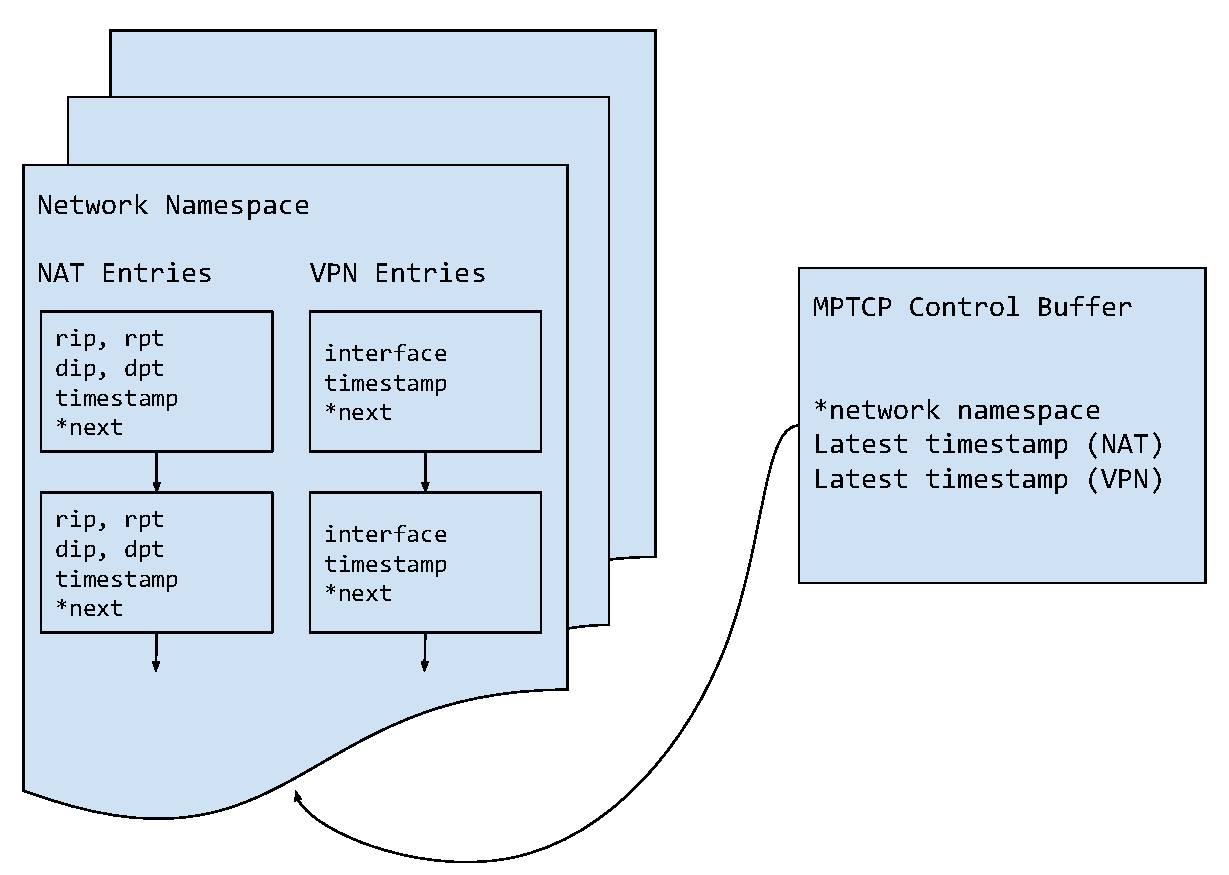
\includegraphics[width=0.8\textwidth]{figures/KernDataStruct.pdf}
  \caption{Simplified view of Path Manager data structures}
  \label{fig:KernDataStruct}
\end{figure}

The path manager receives space within the \ac{mptcp} control buffer to track
state, and it registers a set of callbacks with the protocol, so that it can be
notified of events as they occur. Global state, such as the list of available
detours, must be stored on a per-network namespace basis. This is required not
only to satisfy the demands of a modern kernel which supports namespacing and
containerization, but also so that experiments using Mininet, which relies on
namespaces, run successfully. A simplified view of the data structures
maintained by the path manager is presented in Figure~\ref{fig:KernDataStruct}.

The path manager consists of two main components. First, a subflow worker which
selects and adds detour subflows to an \ac{mptcp} connection. Second, a Generic
Netlink communication interface so that information and commands can be
exchanged with user-space components.

\subsection{Subflow Worker}

The subflow worker runs in two situations, in the context of a particular
\ac{mptcp} socket: (i) when a \ac{mptcp} connection becomes fully established
(i.e. after the three-way handshake completes), and (ii) when a new detour has
been made available to a connection's network namespace, and the detour could be
used for that connection.

When an \ac{mptcp} connection becomes fully established, the subflow worker
starts for the first time. At this point, it uses the Generic Netlink
communication interface (described in Section~\ref{s:genl}) to request a detour
from the client daemon. It does this even if detours are already available, so
that the client daemon may create and report new ones. Then, the path manager
looks through the internal lists of detours in the network namespace of the
socket. The path manager maintains two lists of potential detours per network
namespace. The first is a list of OpenVPN detours. These detour entries are not
specific to a server, and they simply indicate the name of a network interface
to use. The second list contains \ac{nat} detours. These consist of a detour
address and port, and a server address and port. The worker may only select
\ac{nat} entries which match the destination address and port of the current
connection.

The subflow worker then attempts to add up to $N$ subflows, where $N$ is a
configurable limit. The worker may terminate in one of two ways. Either it has
exhaused all of the available detours, but not yet created all $N$ subflows.
Otherwise, if it creates $N$ subflows successfully, it stops looking through the
list, even if more detours are available. When the number of available detours
exceeds $N$, the first $N$ detours, ordered from oldest to newest, are chosen.
If OpenVPN detours are available, then they take precedence over the \ac{nat}
detours, because they are available immediately. \ac{nat} detours are only
available after the successful exchange described in Section~\ref{sec:nat}.

\subsection{Generic Netlink}
\label{s:genl}

In order to request and receive detour entries from userspace, the path manager
relies on a communication interface based on Generic Netlink. Netlink is an
address family for the socket interface (\texttt{AF\_NETLINK}, similar to
\texttt{AF\_INET}), which allows communication between kernel and userspace.
Many existing Linux network configuration utilities communicate with the kernel
over the Netlink address family, such as route and firewall configuration. Each
of the subsystems being configured has a corresponding protocol family, such as
\texttt{NETLINK\_NETFILTER} for Netfilter firewall configuration. These protocol
families take the same place in the \texttt{socket()} system call as protocol
families such as \texttt{IPPROTO\_TCP} in the \texttt{AF\_INET} and
\texttt{AF\_INET6} address families.

Creating a new Netlink protocol involves allocating a new Netlink protocol
family. To make this process easier, the Generic Netlink protocol family was
created. It allows custom protocols (``Generic Netlink families'') to be
created, dynamically allocated, and discovered. It also provides a common format
for sending several data types, and creates a framework for defining message
types. Further, Generic Netlink provides a multicast capability, allowing kernel
and user sockets to broadcast messages to any socket which has joined a
particular multicast group. Finally, Generic Netlink comes with a kernel and
userspace library which allows for a consistent API and a level of abstraction
when defining Generic Netlink families.

We implement a Generic Netlink family, with the following operations
implemented:

\begin{itemize}
\item \texttt{DETOUR\_C\_REQ}: An announcement message sent from the kernel to a
  multicast group, which the client daemon subscribes to. Specifies a remote
  address and port which the kernel would like to create a detour to.
\item \texttt{DETOUR\_C\_ADD}: A command sent from userspace to the kernel that
  adds a detour (of type \ac{nat} or VPN) to the kernel's internal list of
  detours. When a new, unique detour is received, each connection in the
  namespace is informed of the new detour. This gives every connection the
  opportunity to create a subflow along new detours.
\item \texttt{DETOUR\_C\_DEL}: A command sent from userspace to the kernel that
  removes a detour from the kernel's internal list. This does not cancel any
  subflows currently using the detour.
\item \texttt{DETOUR\_C\_ECHO}: A command sent from userspace to the kernel,
  requesting that the kernel write out its list of detours to the kernel log.
  This is a useful command for development and debugging.
\end{itemize}

Generic Netlink provides mechanisms for giving permissions to each operation,
and allows the kernel to work only within the network namespace of the calling
program. As a result, the client daemon may only add or remove detours or
receive requests from its own namespace.

\section{Client Daemon}

The client daemon has two main responsibilities. First, it must create OpenVPN
connections and report them to the kernel. Second, it must respond to detour
requests from the kernel by creating \ac{nat} detours and reporting them back.

The daemon has a configuration file which allows the user to specify the IP
addresses of hosts to use for both types of detours. On startup, the daemon
executes an instance of the OpenVPN client for each configured VPN detour, and
waits for them to fully initialize. The OpenVPN software creates a virtual
network interface which connects to the detour. A new thread is used to monitor
each OpenVPN client process, logging any important messages.

Next the daemon creates a UDP socket corresponding to each \ac{nat} detour in
its configuration file. A separate thread is launched, which calls
\texttt{select()} on the set of detour sockets, waiting for incoming responses
from any detour.

Finally, the detour creates a Netlink socket, subscribes to the path manager's
multicast group, and begins waiting for requests. For each request, it sends a
UDP request to every \ac{nat} detour. When the receiving thread receives a
response, it sends the final \ac{nat} detour information back over the Netlink
socket to the path manager. The path manager may then apply the \ac{nat} detour
to any \ac{mptcp} connections which may use it.

The client daemon may also send \texttt{DETOUR\_C\_DEL} requests to the kernel
in order to clean up older detours. The path manager itself only cleans up
detours when their corresponding network namespace is closed.

\section{Security Considerations}
\label{sec:security}

There are several considerations that must be made for security in this system.
Since detours are along the route of a second subflow, they are able to observe
the destinations of all \ac{mptcp} connections which a client wishes to detour
through them. There is no way to prevent this leak of information, since detours
must know the destination to perform forwarding.

Another serious concern is that detours may record, modify, or forge traffic
between the client and server. This risk exists with routers and middleboxes on
the path of any TCP connection. However, with our system, the detour may be
controlled by an arbitrary user on the network edge, rather than having a
privileged location within the network core.

An application may use TLS on the connection in order to mitigate some of this
risk. The TLS handshake information will be exchanged on the first subflow,
before detour subflows are established. As a result, a detour subflow that
carries TLS will already be fully encrypted, protecting both the privacy of the
connection, and preventing modification.

Applications which do not use TLS are still at risk of attack by a malicious
detour. Small detour collectives made up of individuals with mutual trust could
use the certificate verification features of OpenVPN to protect themselves.
These collectives might create a single root certificate and use that to sign
each member's key. Clients and detours could then authenticate each other as
members of the same collective. However, larger collectives would have to deal
with the same systemic issues that other large-scale \acp{pki} face:
over-privileged intermediates, poor identity verification practices, aging
cryptography, etc \cite{durumeric2013analysis}. An alternative could be a more
distributed web-of-trust model \cite{abdul1997pgp}, but this would require new
authentication mechanisms outside of OpenVPN. In any case, the security of a
detour in a ``Detour Collective'' is still an area requiring future work.

\chapter{Evaluation}
\label{c:eval}

The literature has already established that one-hop overlay routes can improve
connection latency, loss rate, and throughput
\cite{detour,ron,gummadi2004improving}. Therefore, when designing experiments to
evaluate our system, we did not attempt to replicate these results. Instead, we
demonstrate that our system performs as expected, by using proof-of-concept
tests. Specifically, we attempt to answer the following questions:

\begin{itemize}
\item Given a network where an alternative path with better connection
  properties exists, can this mechanism achieve the throughput of the better
  path?
\item Given a network where the core is the bottleneck, rather than access
  links, can this method aggregate the throughput of alternative paths?
\item What overhead exists in this mechanism compared to standard TCP across the
  default route or standard TCP across a detour?
\item What is the difference in the performance of the NAT and VPN detours?
\item Can this mechanism be used across the Internet at higher throughput?
\end{itemize}

We design two types of experiments to answer each of these questions. The first
is based on network emulation, and is designed to answer the first four
questions. The second experiment deploys this mechanism across geographically
distributed hosts, as a proof-of-concept of the mechanism operating on the
Internet.

\section{Mininet Experiments}

Our first set of experiments is based on the Mininet tool \cite{mininet}. As
discussed in Section~\ref{sec:mn}, Mininet is a software-defined networking tool
that allows emulation of large networks on a single machine using the native
operating system networking stack.

\subsection{Fidelity Considerations}

One criticism of the Mininet framework is that in situations with high load, its
timing fidelity (i.e., the accuracy of the performance results) can suffer
\cite{lantz2010network}. Later work has addressed this by allowing users to
limit the CPU utilization of each emulated host, as well as restricting the
bandwidth of links using the Linux traffic control features
\cite{handigol2012reproducible}.

We observed that our test systems could emulate networks with throughput up to
24 Gbps. To ensure that our experiments did not approach the limits of Mininet's
performance fidelity, we limited the bandwidth of each link to no more than
20Mbps, and used relatively few hosts and links. Each host is CPU limited, so
that it may use no more than a tenth of the available processor time. Finally,
we used experiment output provided by IPerf to verify that CPU utilization
remained low during each experiment. In all cases, CPU utilization was no higher
than 5\% over the course of an experiment.

\subsection{Topology}

\begin{figure}[htbp]
  \centering
  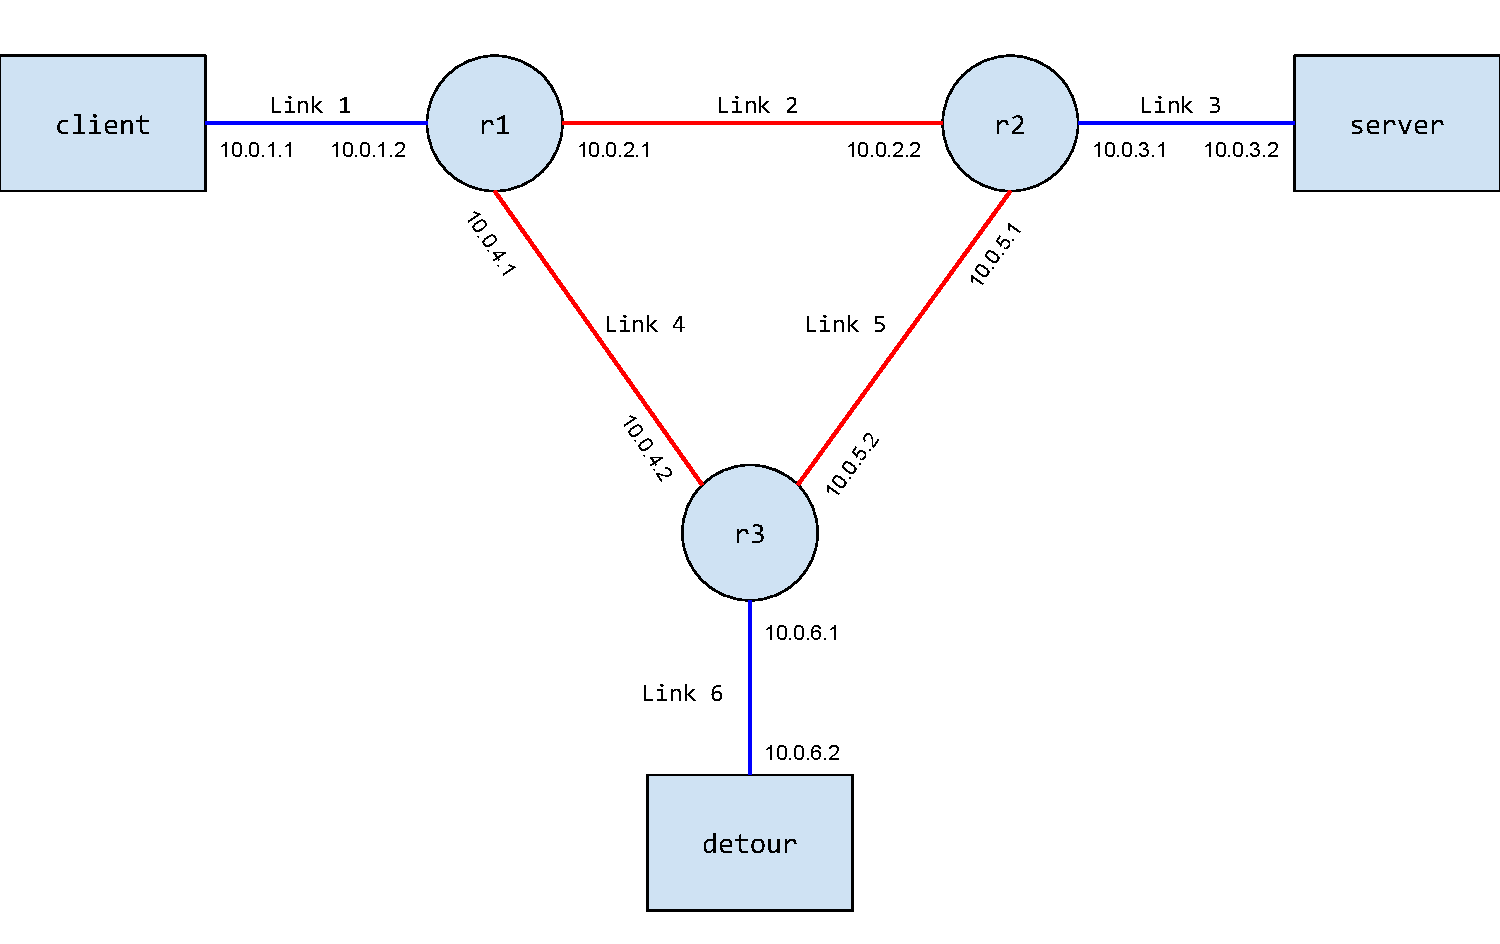
\includegraphics[width=\textwidth]{figures/Topology.pdf}
  \caption[Experimental network topology]{Experimental network topology. Core
    links are highlighted in red. Access links are highlighted in blue.}
  \label{fig:topo}
\end{figure}

Our network topology is illustrated in Figure~\ref{fig:topo}. The routers,
client, server, and detour are Linux hosts, as described in
Section~\ref{sec:mn}. They are statically configured with routes, so that the
default route from \texttt{client} to \texttt{server} traverses Link 2. Routing
is enabled within the Linux kernel.

While configuring routing tables, we encountered issues where Linux kernel
routing rejected incoming packets as ``Martians.'' That is, packets which
originated from an interface which is not the default route for their source
address. To avoid these issues, we disabled Martian filtering in the Linux
kernel. This appears to be an artifact of our test environment, unrelated to the
mechanism.

\subsection{Methodology}

To evaluate the performance of this mechanism, we vary the traffic control
configurations of the links in the topology. There are two main traffic control
configurations tested.

\begin{itemize}
\item \textbf{Symmetric.} The first configuration gives each link the same
  traffic control properties: 10Mbps bandwidth and 5ms delay.
\item \textbf{Core-limited.} The second configuration gives each link within the
  network ``core'' (i.e. links 2, 4, and 5) 10Mbps of bandwidth and a 5ms delay.
  Meanwhile, the access links (i.e. links 1, 3, and 6) are assigned 20Mbps, with
  the same 5ms delay. This aims to simulate a situation in which the access link
  can support more bandwidth than the default Internet path can support.
\end{itemize}

We chose 10Mbps links for two reasons. First, lower capacity links emulate the
scenario where the network core can only provide a fraction of capacity to one
connection. Second, lower capacity links keep the total throughput of the system
well under the limitations of our test system, ensuring accurate emulation. For
each traffic control configuration, we also create two modifications.

\begin{itemize}
\item \textbf{Lossy.} Link 2 is configured to drop packets independently and
  randomly with probability 0.01. This is within the range of packet loss rates
  Savage \textit{et al.} observe over ``bad'' paths in their Detour study
  \cite{detour}. We ran smaller experiments with loss rates of 0.5\%, 2\%, and
  5\%, with similar results to the ones presented here.
\item \textbf{Delayed.} Link 2 is configured to have a high (100ms) latency. We
  also tested latencies of 20ms and 50ms, although 100ms was the first to show
  observable differences in throughput.
\end{itemize}

This results in a total of six traffic control configurations. For each traffic
control configuration, we use the standard IPerf 3 tool to measure \ac{mptcp} or
TCP throughput between \texttt{client} and \texttt{server}. We test the
following procedures:

\begin{itemize}
\item \textbf{1-Subflow.} MPTCP is enabled, but no detours are configured on the
  client. The connection uses only one subflow, across the Internet routed path.
\item \textbf{\ac{nat}.} In addition to a subflow on the Internet routed path, a
  second subflow is through a \ac{nat} detour.
\item \textbf{OpenVPN.} In addition to a subflow on the Internet routed path, a
  second subflow is through a OpenVPN detour.
\item \textbf{TCP.} MPTCP is disabled. A regular TCP flow is used, across the
  default Internet routed path. The default Linux congestion control (CUBIC) is
  used.
\item \textbf{\ac{nat} TCP.} A regular TCP flow is used, but it is directed
  through the NAT detour.
\item \textbf{OpenVPN TCP.} A regular TCP flow is used, but it is directed
  through the VPN detour.
\end{itemize}

Throughput is measured with a 10 second IPerf session, which involves
transmitting as much data as possible over a TCP (or \ac{mptcp}) connection. 10
seconds is the default interval for an IPerf session. In our experiments, the
TCP flows reached their peak throughput within less than a second. Since
\ac{mptcp} has a slower mechanism for closing a connection than standard TCP,
\ac{mptcp} IPerf sessions lasted a few seconds longer than the TCP sessions.
During these final time intervals, the data throughput slowed down
significantly, contributing significant variation to our results. In order to
control for these factors, we filter out the first second and any time intervals
after 10 seconds. Thus, for each trial, we measure the throughput as the number
of bytes transmitted during these 9 seconds, divided by 9 seconds. We ran 60
trials for each combination of parameters.

\subsection{Results}

\begin{figure}[htbp]
  \centering
  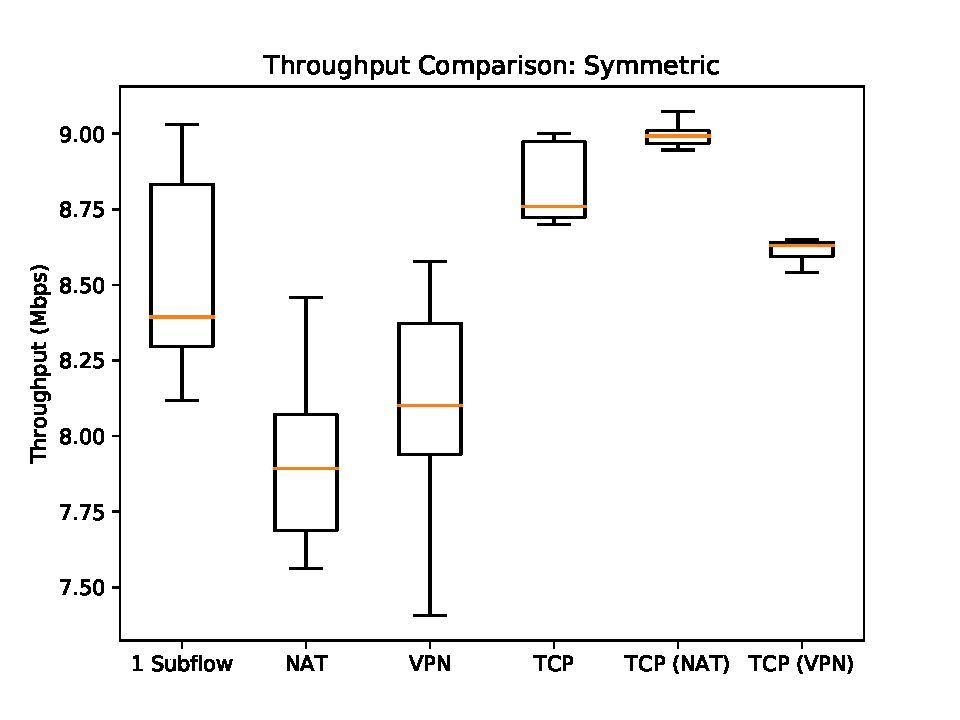
\includegraphics[height=0.42\textheight]{figures/sym.pdf}
  \caption{Throughput Comparison: Symmetric}
  \label{fig:sym}
\end{figure}

Figure~\ref{fig:sym} shows a performance comparison of the mechanism on the
Symmetric network without loss or latency. In this figure, each distribution is
represented by a box outlining the first and third quartiles of the data, with a
line through the center representing the median. The whiskers show the spread of
the data, and points outside of 1.5 times the interquartile range are marked
with circles as outliers. The data shown in this and all subsequent
box-and-whisker plots of this section are also given in tabular form in
Table~\ref{t:d} in the Appendix.

In this configuration, we can see four important pieces of information. First,
we observe the overhead of single-subflow \ac{mptcp} compared to TCP to be
around 140kbps in this scenario. This amounts to a 1.5\% loss in throughput.
This overhead is due to the presence of the \ac{dss} option in each segment. In
packet captures, we observed that the Linux \ac{mptcp} implementation tends to
send a \ac{dss} option with every data packet, and that these options are
usually 20 bytes. On TCP segments with MSS of 1460, this amounts to 1.37\% of
the MSS. So, the observed \ac{mptcp} overhead is in line with expectations.

Second, by comparing the TCP and TCP (NAT) throughputs, we can observe the
overhead inherent in the \ac{nat} mechanism when compared to TCP over the
default route. This overhead will of course vary depending on topology, but the
added processing incurred by the \ac{nat} detour mechanism must be less than
this overhead. We see about 200kbps overhead, or around 2\%.

Third, by comparing the TCP and TCP (VPN) throughputs, we can observe the
overhead inherent in the VPN mechanism when compared to TCP over the default
route. We see a much greater overhead of 630kbps, or 6.6\%. In packet captures,
we observed that the MSS of normal TCP segments was 1428, while the MSS of TCP
segments transmitted through OpenVPN was 1337, leaving 91 bytes of overhead.
This amounts to 6.4\% of the segment size. So, again, the observed in OpenVPN is
in line with expectations.

Fourth, we can see that \ac{mptcp} with the \ac{nat} detour performs identically
to 1-Subflow \ac{mptcp}, even though the two subflows of this mechanism must
compete for the access link capacity. Due to the increased overhead of the VPN
approach, \ac{mptcp} with the VPN detour does not perform as well. However, the
difference is smaller than the difference between TCP and TCP (VPN), since the
subflow on the default path makes up for some of the overhead.

\begin{figure}[htbp]
  \centering
  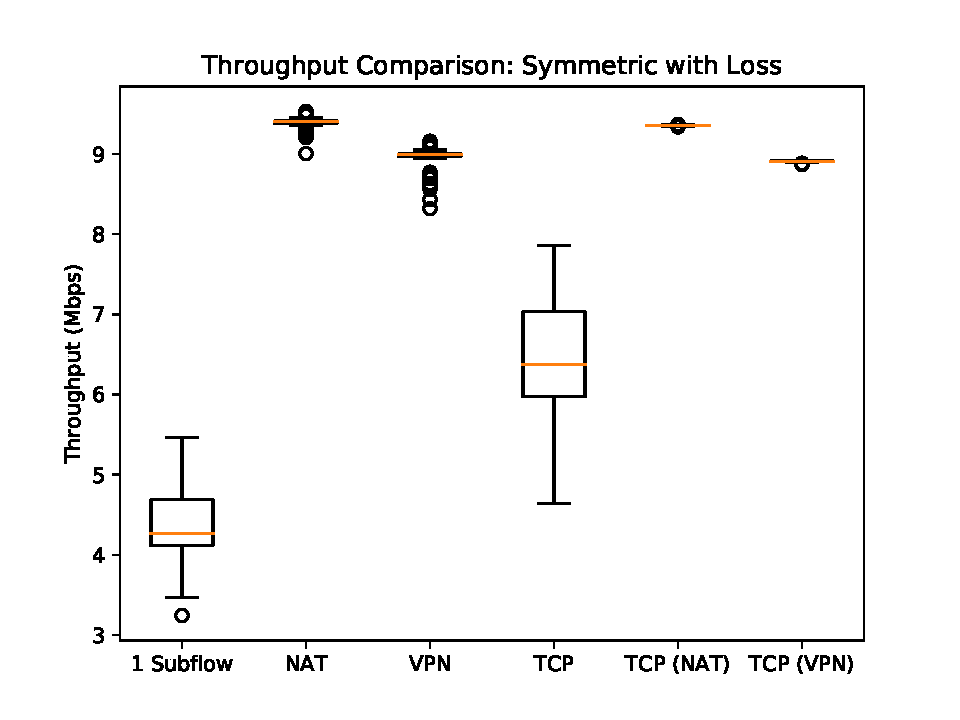
\includegraphics[height=0.42\textheight]{figures/sym-lossy.pdf}
  \caption{Throughput Comparison: Symmetric, with Loss}
  \label{fig:sym_lossy}
\end{figure}

In Figure~\ref{fig:sym_lossy}, we see the effect of adding a 1\% loss rate to a
link that is present only on the default path. Regular TCP and \ac{mptcp} with
one subflow show significant losses in throughput, and much more variable
throughput as well. Under loss, \ac{mptcp} performs worse relative to TCP
because its \ac{lia} congestion control is more conservative than the CUBIC
congestion control used by regular TCP.

\ac{mptcp} with \ac{nat} very slightly outperforms TCP (NAT), and \ac{mptcp}
with VPN very slightly outperforms TCP (VPN). In both cases, the difference is
not statistically significant. In fact, \ac{mptcp} with detours shows much more
variability (standard deviations of 0.08 and 0.17 for \ac{nat} and VPN
respectively). This is because the variability of the subflow along the default
route adds variability to the overall connection.

\begin{figure}[htbp]
  \centering
  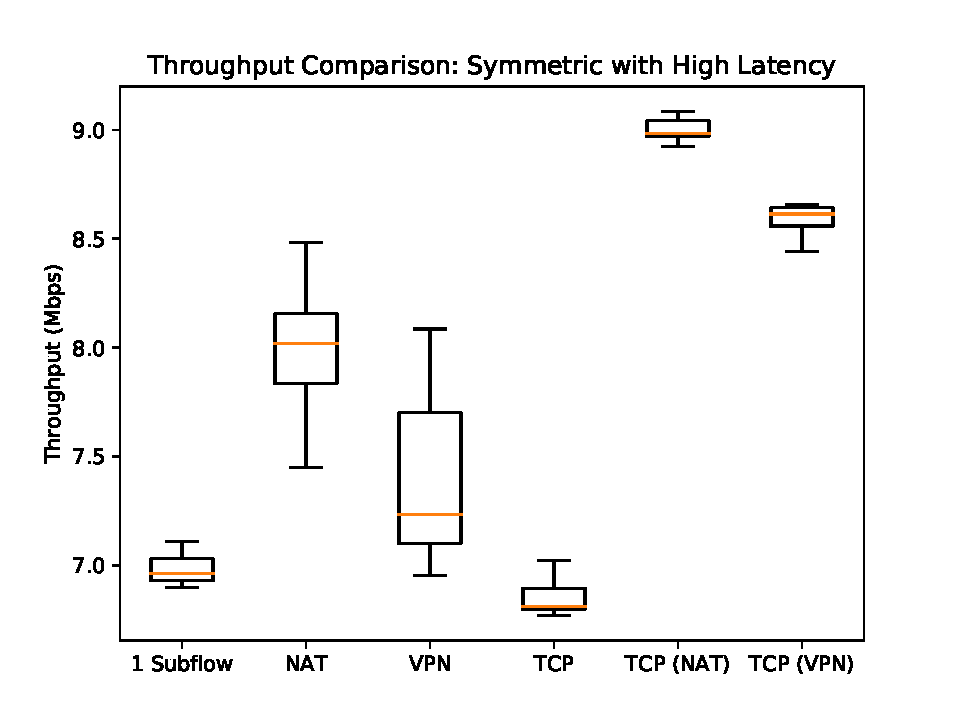
\includegraphics[height=0.42\textheight]{figures/sym-delayed.pdf}
  \caption{Throughput Comparison: Symmetric, with Latency}
  \label{fig:sym_delayed}
\end{figure}

In Figure~\ref{fig:sym_delayed}, we see the impact of the high latency link
along the default route. The performance of 1-Subflow \ac{mptcp} and standard
TCP suffers due to the increased round trip time. \ac{mptcp} with the \ac{nat}
detour is able to achieve a similar throughput to TCP (NAT), since the Lowest
RTT first scheduler routes 82.3\% of the data across the detour subflow.
\ac{mptcp} with the VPN detour demonstrates unusual behavior. Despite the
increased latency of the default route, only 48.0\% of data is scheduled across
the VPN detour, suggesting that the VPN adds a significant amount of latency.

\begin{figure}[htbp]
  \centering
  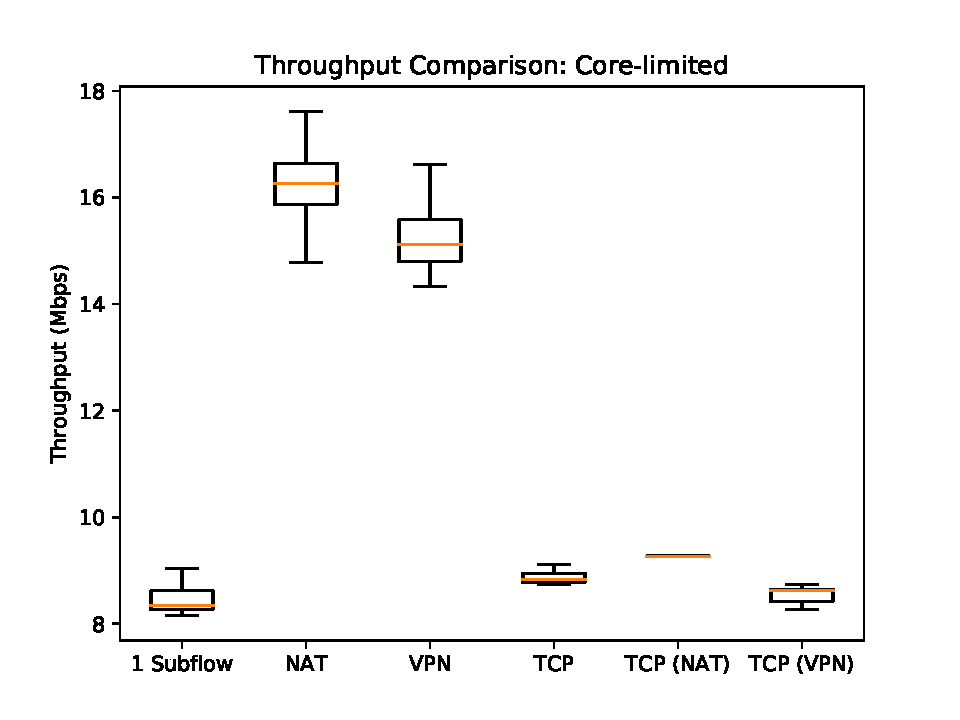
\includegraphics[height=0.42\textheight]{figures/easy.pdf}
  \caption{Throughput Comparison: Core-limited}
  \label{fig:easy}
\end{figure}

The results for the core-limited network are much different.
Figure~\ref{fig:easy} shows a comparison of throughput on the core-limited
network, with no loss or latency. Since the detour path traverses different core
links than the default path, there is no competition. Thus there is the
potential to aggregate the capacity of both paths. The \ac{nat} detour achieves
98.5\% of the sum of the throughputs of TCP and TCP (NAT). The VPN detour
obtains a 98.1\% of the sum of the throughputs of TCP and TCP (VPN). Again, the
\ac{nat} detour performs better than the VPN detour due to the packet overhead
of OpenVPN.

\begin{figure}[htbp]
  \centering
  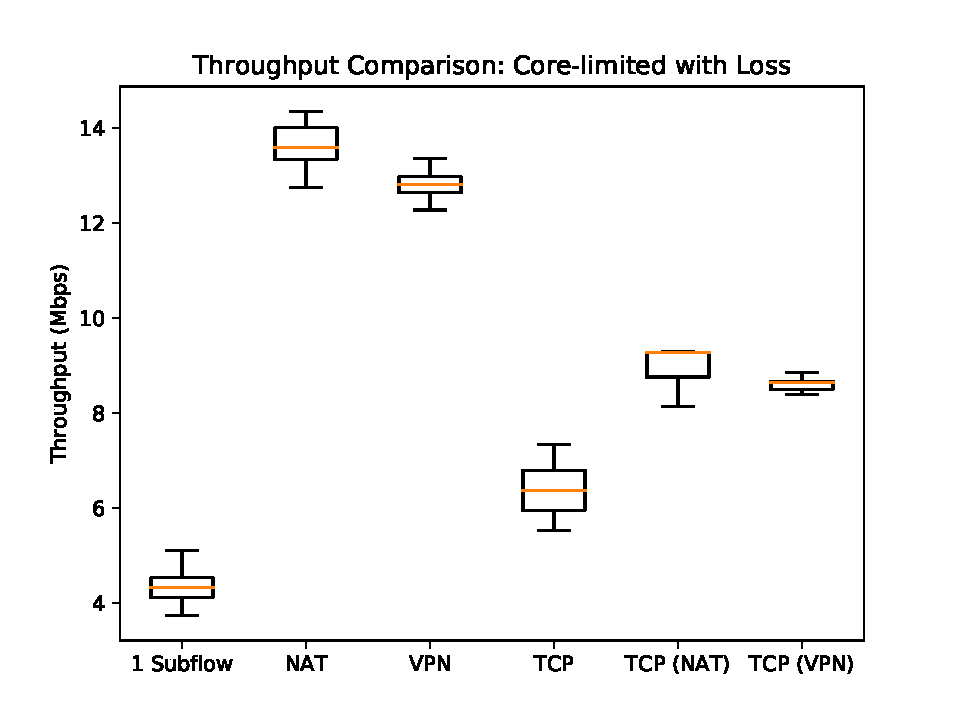
\includegraphics[height=0.42\textheight]{figures/lossy.pdf}
  \caption{Throughput Comparison: Core-limited, with Loss}
  \label{fig:lossy}
\end{figure}

When loss is introduced, Figure~\ref{fig:lossy} shows that the \ac{nat} and VPN
methods outperform their pure TCP variants, since they are able to aggregate the
throughput of both paths. Even though the default path is lossy, it is able to
contribute some throughput to the \ac{mptcp} connection.

\begin{figure}[htbp]
  \centering
  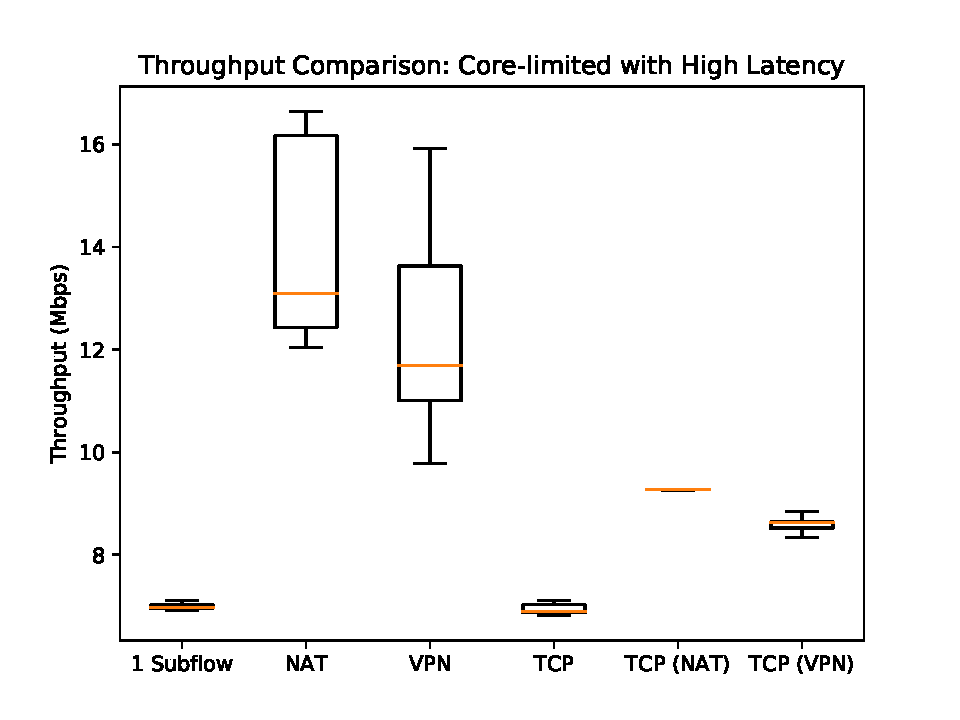
\includegraphics[height=0.42\textheight]{figures/delayed.pdf}
  \caption{Throughput Comparison: Core-limited, with Latency}
  \label{fig:delayed}
\end{figure}

Similarly, when latency is introduced, Figure~\ref{fig:delayed} shows that the
\ac{nat} detour continues to aggregate throughput, although with slightly more
variability. The VPN detour again demonstrates unusual behavior. In some trials,
the VPN had a very high round trip time, resulting in a long slow-start period
and very low connection throughput. We believe this could be due to an artifact
of our testing framework.

\subsection{Summary}

By emulating a network with varying conditions, we were able to verify that the
mechanism works as expected. By directing subflows across detour routes,
\ac{mptcp} is able to achieve path bandwidth aggregation in some cases. In
situations where no benefit can be achieved by bandwidth aggregation, the
mechanism incurs at least a 1.5\% overhead due to \ac{mptcp} signaling. This
overhead quickly is overcome when loss or latency is added to one of the paths.
When path bandwidth aggregation is possible, the mechanisms are capable of
aggregating over 98\% of the sum of the throughputs achieved by TCP across both
paths.

Across all the connections, the \ac{nat} approach performs slightly better than
the VPN, due to the additional overhead of the IP and UDP encapsulation, along
with OpenVPN protocol overhead and latency.

\section{AWS Experiment}

The Mininet experiments demonstrate that this method can indeed circumvent lower
quality paths, and also aggregate the capacity of different paths through the
network. However, these experiments run on a single platform: client, server,
detour, and routers all share the same network stack. The real Internet is much
more heterogeneous. To demonstrate the feasibility of this mechanism on the wide
area Internet, we designed a full-scale experiment.

Using Amazon Web Services' Elastic Cloud Compute service (AWS EC2), we deployed
three instances of type \texttt{m4.large}, each in a different region. The
client is located in the \texttt{us-west-1} region (Northern California), the
detour in \texttt{us-east-2} (Ohio), and the server in \texttt{us-east-1}
(Northern Virginia). We then ran the IPerf 3 tool for 100 trials in each of the
same configurations as the previous experiments.

\begin{figure}
  \centering
  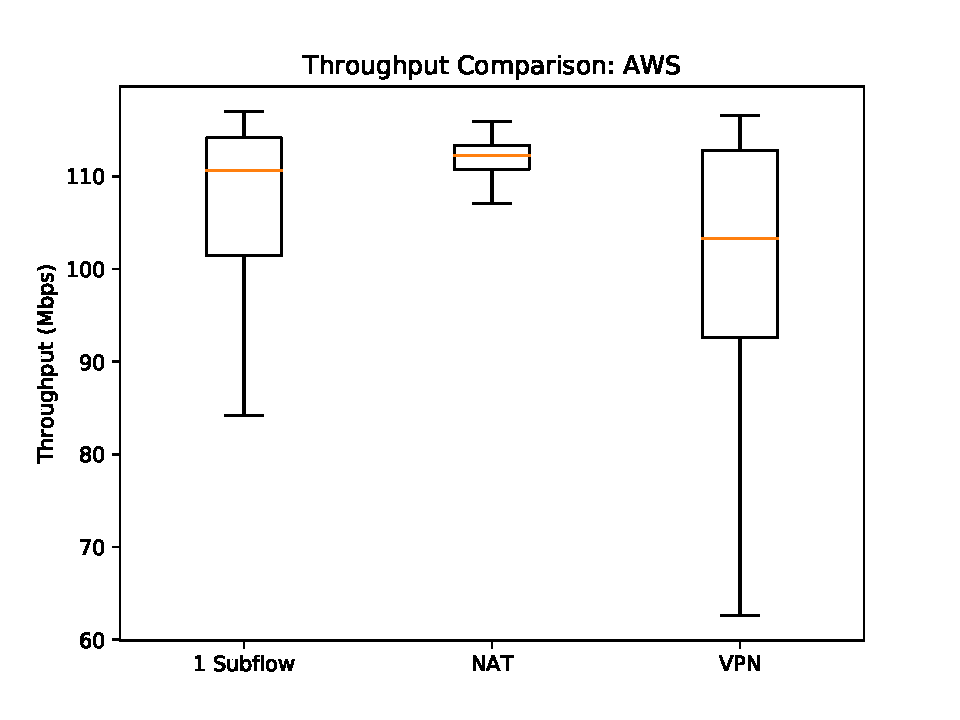
\includegraphics[height=0.45\textheight]{figures/aws.pdf}
  \caption{Throughput Comparison: AWS}
  \label{fig:aws}
\end{figure}

Figure~\ref{fig:aws} shows a throughput comparison. The connections were able to
achieve a much higher throughput than in the emulated networks. None of the
\ac{mptcp} based configurations were able to outperform standard TCP. The most
important result of this experiment is that standard TCP across the VPN detour
is not capable of achieving more than about 60Mbps, due to the increased
processing overhead of OpenVPN. As a result, in terms of capability to enable
high throughput transfers, the \ac{nat} detour is a better choice.

\chapter{Future Work}
\label{c:fw}

The mechanisms described in this thesis are the foundation for a much larger
system, with many problems that must be solved before it can be generally
deployable. In this chapter, we discuss these problems and other potential
extensions to our work.

\section{Detour Collective}

One fundamental question regarding the deployment of this mechanism has not yet
been addressed: where are detour hosts found, and what is their motivation for
forwarding traffic? One possibility is that a group of users could form a group
that aims to help each other improve their connection quality. Some form of
protocol, either centralized or decentralized, could allow users to join,
offering their computer as a detour, in return for the use of other detour
hosts.

Ultimately, this group would be very similar to the overlay networks described
previously. However, unlike most of these, the overlay network would be
restricted to single hop source routing of \ac{mptcp} connections.

The VPN detouring mechanism would be particularly conducive to such a
collective. The OpenVPN protocol uses a PKI for authentication of client and
server. So, a centralized collective could use this PKI to enforce membership
cryptographically. When a user joins, they generate a private key and request
that the central authority sign it. By using the central authority's certificate
as a PKI root, they may ensure that only members of the collective could use
their detouring services. By having their private key signed, users could gain
access to the detouring services of other members.

Another possibility for deployment could be through ISPs. While the
inefficiencies created by policy routing on the Internet motivate this work,
ISPs must also continue differentiating themselves to remain competitive to
consumers. For example, Korea Telecom has launched an \ac{mptcp}-based proxy
system to provide gigabit Internet speeds to smartphone users, and the IETF is
currently discussing a draft about \ac{mptcp} proxying by ISPs
\cite{boucadair-mptcp-plain-mode-10}. As a result, ISPs may also be interested
in improving customer experience by implementing a detour system. An ISP could
place detour points at several places in its network, and distribute detour
information to customers via a centralized protocol. In this case, clients would
not need to provide detouring services to each other, because the ISP provides
them. Further, competing ISPs could federate detour systems (similar to peering
agreements) so that their customers could gain access to better-situated detour
points.

\section{Detour Traffic Attribution}

Similar to exit nodes in Tor \cite{tor}, detours act as exit points for unknown
traffic. In both cases, traffic bound for the Internet must undergo \ac{nat},
with the source address being replaced with the exit point's address. Thus,
traffic emerging from a Tor exit or a detour can be wrongly attributed as
originating from that host. Depending on the nature of the traffic, this can be
dangerous for the exit node, as they could be held responsible for illegal
activity. As a result, running a detour represents some risk.

One potential mitigating factor could be the use of client certificates in the
OpenVPN detour authentication process. By authenticating each other, a Detour
can have cryptographically verified information about the client which will be
using its services, assuming that this information is included in the
certificate. Combined with detailed logging of outgoing connections, a Detour
may accurately attribute connections to their source, providing strong evidence
of innocence in the event of an investigation.

Furthermore, while the goal of Tor is providing anonymity, the goal of our
detour mechanism is improving performance and reliability. The anonymity
provided by Tor is a lucrative resource to those using the Internet for illegal
activity, and our service provides no such guarantee. As a result, the risks
associated with running a detour are much lower than running a Tor exit node.
However, these arguments do not fully address the traffic attribution problem,
and future consideration is necessary for a full deployment of our mechanism.

\section{Dynamic Source Routing}

In the \ac{ron} system, overlay routing is performed at each node \cite{ron}.
Similarly, the Detour study describes a system in which routing is performed at
each overlay node \cite{detour}. In our system, we apply source routing. While
overlay routing mechanisms have been described for systems like \ac{ron} and
Detour, we are unaware of algorithms which attempt to find the best route for a
packet from its source, with incomplete knowledge of the capacity and state of
the network links.

An extension to this work would be to extend it with such an algorithm. This
algorithm would maintain several \ac{mptcp} subflows, and every so often it
would decide to close one in favor of a new route. This decision would have to
take into account at least the following factors:

\begin{itemize}
\item \ac{rtt} and observed loss rate of the subflow considered for eviction.
\item Change in \ac{rtt} and observed loss rate of the other subflows since this
  one was added.
\item Potentially outside observations, such as statistics from other subflows,
  or statistics generated from userspace monitoring programs.
\end{itemize}

Together with a Detour Collective, this could almost completely automate the
process of using this framework for an end user.

\section{Data Scheduling}

The kernel modifications of this framework currently only consist of a path
manager. We have no control of the scheduling of data across the subflows we've
created, beyond selecting an appropriate scheduler. An extension of this work
could be to implement a data scheduler for the framework. A custom scheduler
could send data redundantly across new subflows just after they are added, so
that there is no loss in reliability when assessing the performance of a new
subflow. Further, a scheduler could detect whether a particular flow is
application limited or network limited, and schedule differently based on this.
For instance, redundantly sending data across each subflow could improve overall
latency and loss rates, but it would only make sense when the connection is
application limited. A network limited connection would be best served by a less
wasteful strategy, such as the default Lowest \ac{rtt} First scheduler.

\section{0-RTT NAT Establishment}
\label{sec:0rtt-nat}

Currently, the \ac{nat} forwarding mechanism uses a UDP-based protocol for
requesting tunnels. This protocol is rather naive and vulnerable to many obvious
exploits. While future work is required to harden this protocol, there are other
possibilities which could eliminate the 1-RTT required to establish a NAT
mapping. Since the NAT detouring mechanism has less space overhead, and
therefore a measurable improvement over the VPN detour, eliminating this 1-RTT
delay would remove the tradeoff between startup speed and overall throughput.

One possibility may be to embed the final destination of the initial
\texttt{SYN} packet into an IP option. This would eliminate the need for a
signaling protocol. This would require implementing a Netfilter module for the
detour host's kernel. However, Medina \textit{et al.} \cite{medina2005measuring}
measure that 70\% of TCP SYN packets carrying an unknown IP option are dropped.
Additionally, Fonseca \textit{et al.} \cite{fonseca2005ip} measure that half of
packets containing IP options are dropped. While it is possible that these 2005
findings are no longer accurate, further investigation is required before
investing in a solution based on IP options.

Another possibility is to create a TCP option containing the destination
address, and add it to the initial SYN. \ac{mptcp} requires TCP options in order
to function, so TCP options would not incur the same compatibility concerns that
IP options do. Yet another possibility is including the final destination within
a data element of the TCP SYN packet. This strategy is used in the IETF's
\ac{mptcp} proxying draft \cite{boucadair-mptcp-plain-mode-10} as a way to
communicate the final destination of a SYN packet. In either of these cases, it
is likely that kernel modifications would be necessary for the detour host.

\chapter{Conclusion}
\label{c:conclusion}

In this thesis, we have described the implementation and evaluation of a system
for adding non-default paths to \ac{mptcp} connections. We implemented this as a
path manager in the 0.91 version of the Multipath TCP Linux kernel, along with
several user-space utilities which complete the system.

The implementation is structured so that two different mechanisms for tunneling
subflows are allowed. We have seen that the \ac{nat} approach has slightly
better performance due to its lower space and processing overhead. However, that
increased performance comes at the expense of an extra \ac{rtt} for setting up a
tunnel, and the extra complexity of a dynamic client which creates them. The VPN
approach is simpler, but has higher overhead.

When compared to standard TCP over the best available path, this mechanism
incurs a modest overhead when the same bottleneck link is present on both paths.
However, when the paths have separate bottlenecks, this mechanism is capable of
aggregating the bandwidth of both paths, achieving better performance than
standard TCP across the best path.

This mechanism is compatible with unmodified applications on the wide area
Internet today. We believe that as high-bandwidth access links become more
common, the collaborative bandwidth sharing systems this enables will become
more relevant. In the meantime, there are several opportunities for extending
this work and using it to study problems like detour routing.

\backmatter
\appendix

\chapter{Data}

\begin{table}[H]
\resizebox{\columnwidth}{!}{%
\begin{tabular}{l|rrrrrr}
   & \textbf{1 Subflow} & \textbf{NAT} & \textbf{VPN} & \textbf{TCP} & \textbf{TCP (NAT)} & \textbf{TCP (VPN)}\\
  \hline
(*)Core-limited & 9.41 (0.01) & 18.81 (0.02) & 18.30 (0.18) & 9.55 (0.00) & 9.55 (0.01) & 9.11 (0.01) \\
Core-limited, 0.5\% Loss & 9.42 (0.00) & 18.83 (0.01) & 18.27 (0.34) & 9.54 (0.01) & 9.55 (0.01) & 9.12 (0.01) \\
(*)Core-limited, 1\% Loss & 4.21 (0.34) & 13.76 (0.38) & 13.05 (0.48) & 6.16 (0.61) & 9.55 (0.00) & 9.11 (0.01) \\
Core-limited, 2\% Loss & 2.89 (0.25) & 12.36 (0.29) & 11.60 (0.38) & 4.17 (0.42) & 9.54 (0.01) & 9.10 (0.01) \\
Core-limited, 5\% Loss & 1.50 (0.14) & 11.01 (0.14) & 10.42 (0.12) & 2.13 (0.19) & 9.55 (0.01) & 9.11 (0.01) \\
Core-limited, 20ms Delay & 9.42 (0.00) & 18.83 (0.01) & 18.28 (0.33) & 9.55 (0.01) & 9.54 (0.01) & 9.11 (0.01) \\
Core-limited, 50ms Delay & 9.42 (0.01) & 18.63 (0.16) & 17.99 (0.21) & 9.55 (0.00) & 9.55 (0.01) & 9.11 (0.01) \\
(*)Core-limited, 100ms Delay & 9.09 (0.01) & 17.73 (0.28) & 15.41 (2.24) & 9.22 (0.01) & 9.55 (0.01) & 9.11 (0.01) \\
(*)Symmetric & 9.41 (0.01) & 9.41 (0.01) & 9.14 (0.03) & 9.54 (0.03) & 9.35 (0.01) & 8.91 (0.00) \\
Symmetric, 0.5\% Loss & 9.42 (0.00) & 9.41 (0.02) & 9.15 (0.04) & 9.55 (0.01) & 9.35 (0.01) & 8.90 (0.01) \\
(*)Symmetric, 1\% Loss & 4.36 (0.44) & 9.39 (0.08) & 8.93 (0.17) & 6.45 (0.68) & 9.35 (0.01) & 8.91 (0.01) \\
Symmetric, 2\% Loss & 2.89 (0.26) & 9.30 (0.17) & 8.85 (0.24) & 3.92 (0.49) & 9.35 (0.01) & 8.92 (0.01) \\
Symmetric, 5\% Loss & 1.47 (0.17) & 9.24 (0.20) & 8.78 (0.25) & 2.10 (0.26) & 9.35 (0.01) & 8.90 (0.02) \\
Symmetric, 20ms Delay & 9.42 (0.00) & 9.42 (0.00) & 9.13 (0.04) & 9.55 (0.00) & 9.36 (0.00) & 8.92 (0.00) \\
Symmetric, 50ms Delay & 9.42 (0.00) & 9.41 (0.01) & 9.23 (0.04) & 9.55 (0.01) & 9.36 (0.01) & 8.92 (0.00) \\
(*)Symmetric, 100ms Delay & 9.10 (0.01) & 9.37 (0.02) & 9.03 (0.09) & 9.22 (0.01) & 9.35 (0.01) & 8.90 (0.03) \\
\end{tabular}
}
\caption[Mininet experiment throughput]{
  Full Mininet throughput data. All units are Mbps (mega bits per second).
  Standard deviation in parentheses. Rows marked with (*) have 60 trials, other
  rows have 20 trials. Values are in the form ``mean (standard deviation)''.
}
\label{t:d}
\end{table}

\begin{table}[H]
  \resizebox{\columnwidth}{!}{%
  \begin{tabular}{l|rrrr}
  Configuration              & Bytes, Default & Bytes, Detour & Percent, Default & Percent, Detour\\
  \hline
  Core-limited, NAT          & 12833473 & 12784884 & 50.09\% & 49.91\% \\
  Core-limited, VPN          & 12752000 & 9446808 & 57.44\% & 42.56\% \\
  Core-limited, Lossy, NAT   & 5881969 & 12039468 & 32.82\% & 67.18\% \\
  Core-limited, Lossy, VPN   & 5607324 & 8957956 & 38.50\% & 61.50\% \\
  Core-limited, Delayed, NAT & 12572613 & 11800992 & 51.58\% & 48.42\% \\
  Core-limited, Delayed, VPN & 12558642 & 10273609 & 55.00\% & 45.00\% \\
  Symmetric, NAT             & 6997237 & 6083280 & 53.49\% & 46.51\% \\
  Symmetric, VPN             & 10655479 & 2638377 & 80.15\% & 19.85\% \\
  Symmetric, Lossy, NAT      & 859693 & 11737856 & 6.82\% & 93.18\% \\
  Symmetric, Lossy, VPN      & 1885375 & 8912407 & 17.46\% & 82.54\% \\
  Symmetric, Delayed, NAT    & 2380513 & 11062716 & 17.71\% & 82.29\% \\
  Symmetric, Delayed, VPN    & 6502281 & 5990180 & 52.05\% & 47.95\% \\
  \end{tabular}
  }
  \caption[Bytes transmitted across subflows]{Bytes transmitted across subflows.
  Measured from 1 trial in each of the configurations, via packet captures.}
\end{table}

\bibliographystyle{ieeetr}
\bibliography{paper}

\end{document}
